% replace all text with your own text.
% in this template few examples are mention
%%%%%%%%%%%%%%%%%%%%%%
\chapter{Problem A}
\label{ch:problem_A}
%

%



\section{Problem Description}

Problem A consists in recovering the Young's modulus $k(x)$ of a 1D rod made of a linearly elastic material given noisy measurements of its displacement field $u(x)$. The Young's modulus is not homogeneous along the length of the rod. The PDE governing this system is

\begin{equation}
	-\frac{d}{dx} \left( k(x) \frac{du}{dx} \right) = f, \quad x \in (0, L)
\end{equation}

\noindent
where $f = 9.81$ is the axial load applied to the rod and $L = 1$ is the rod's length.

The rod's displacement is fixed at both ends, and therefore the PDE is subject to the folling initial conditions:

\begin{equation}
	u(0) = u(L) = 0
\end{equation}

This problem can be categorized as an inverse problem, since we are given observations of the solution $u(x)$ of the PDE and are asked to find the material field $k(x)$, instead of the other way around (which would be deemed a forward problem).

%
\section{Methodology}
%
\subsection{The method selection}


%Describe the method you use and the reason for choosing it.
%
%Method = VPINN
%
%Reason for choosing method = Capable of doing inverse problem naturally (which this one is), also rules out Deep Ritz. DNO's are ruled out since there is only one material field, we're not learning an operator. Performs well on low dimensions (here dim = 1).
%
%Why VPINN specifically? --> By inspecting the noisy u(x) data we can see that it has a simple geometry, therefore the VPINN may be well-suited for this task. Additionally, both ParticleWNN and WAN were tried but VPINN gave the best performance.

%%%%%%%

The method chosen for this problem is to use a Variational Physics-Informed Neural Network (VPINN). This type of neural network is chosen due to its applicability to inverse problems, as opposed other deep learning methods like Deep Ritz, in which inverse problems are not directly possible. Since we are solving for a single material field, it is not necessary to learn an operator. Thus, Deep Neural Operators (DNOs) do not fit this type of problem.

A simple visual inspection of the noisy $u(x)$ data reveals it has a simple geometry, which VPINNs are known to perform well on due to their global polynomial basis. Furthermore, the problem was also attempted using a Weak Adversarial Network (WAN) approach and a Particle Weak Neural Network (ParticleWNN) approach, but the VPINN approach was found to give the best performance on the problem. Additionally, the problem is 1-dimensional, making VPINN a competitive option for this task, as well as making it simple to implement. The reasons listed above make VPINN an excellent method in comparison to other physics-informed methods for this specific problem.

%
\subsection{The loss function}

%Describe the loss function you use and the corresponding hyperparameters (i.e., loss weights, collocation points/integral points, and so on) used in training.

The loss function used for this task is composed of 3 terms: A boundary loss, an observation loss and PDE loss. The boundary loss enforces that the boundary conditions $g(x)$ are satisfied by $u_\theta (x)$, and is defined as

\begin{align}
	\mathcal{L}_\mathrm{bd} &= \frac{1}{N_\mathrm{bd}} \sum_{i=1}^{N_\mathrm{bd}} \left| u_\theta (x_i) - g(x_i) \right|^2 \\
	&= \frac 12 \left| u_\theta (0) - 0 \right|^2 + \frac 12  \left| u_\theta (L) - 0 \right|^2
\end{align}

\noindent
where $N_\mathrm{bd} = 2$ since there are 2 boundary points in the domain.

The observation loss ensures that the network's prediction $u_\theta (x)$ stays consistent with the noisy measurements $u^\mathrm{obs}$ at the sensor locations $x^\mathrm{obs}$. It is defined as

\begin{align}
	\mathcal{L}_\mathrm{obs} &= \frac{1}{N_\mathrm{obs}} \sum_{i=1}^{N_\mathrm{obs}} \left| u_\theta (x_i^\mathrm{obs}) - u_i^\mathrm{obs} \right|^2
\end{align}

\noindent
where $N_\mathrm{obs} = 500$ since there are 500 noisy observations.

Finally, the PDE loss ensures that the pair of predicted functions ($u_\theta (x)$ and $k_\theta (x)$) satisfy the governing PDE. It is computed as the sum of squared weak residuals $R_n$ of each test function $v_n(x)$ for $n = 1, \dots, N_\mathrm{test}$, where $v_n(x)$ is the $n^\text{th}$ Legendre polynomial. The residuals are given by the weak form of the PDE, which is approximated numerically by Gauss-Legendre quadrature.

\begin{align}
	R_n &= \int_{0}^{L} \left( k_\theta(x) \nabla u_\theta(x) \nabla v_n(x) - f(x) v_n(x) \right) dx \\
	&\approx \sum_{j=1}^{N_\mathrm{int}} \left( k_\theta (x_j) \nabla u_\theta(x_j) \nabla v_n(x_j) - f(x_j) v_n(x_j) \right) w_j
\end{align}

\noindent
where $N_\mathrm{int}$ is the number of integral points to use in the quadrature, chosen here to be $N_\mathrm{int} = 100$, and $w_j$ are the quadrature weights.

The PDE loss is then given by

\begin{align}
	\mathcal{L}_\mathrm{PDE} &= \frac{1}{N_\mathrm{test}} \sum_{i=1}^{N_\mathrm{test}} R_i^2
\end{align}

\noindent
The number of test functions $N_\mathrm{test}$ is chosen here to be $N_\mathrm{test} = 100$.

The total training loss $\mathcal{L}_\theta$ is computed as a weighted sum of the 3 losses mentioned previously, where the weights associated to each loss are hyperparameters.

\begin{equation}
	\mathcal{L}_\theta = w_\mathrm{bd} \mathcal{L}_\mathrm{bd} + w_\mathrm{obs} \mathcal{L}_\mathrm{obs} + w_\mathrm{PDE} \mathcal{L}_\mathrm{PDE}
\end{equation}





%
\subsection{The network structure}
%Describe the network structure that you use during training. You can also use a table as follows:
%

The network structure used consists of 2 Multilayer Perceptrons (MLPs), one for the estimation of the Young's modulus $k(x)$ and the other for the estimation of the displacement $u(x)$. Both networks are trained simultaneously during the training process. The network architectures of said MLPs can be found in Table \ref{tab:problem_A_network_k} and Table \ref{tab:problem_A_network_u}.


\begin{table}[H]
\centering
\caption{Architecture of MLP for $k(x)$}
\label{tab:problem_A_network_k}
\begin{tabular}{llll}
\hline
\textbf{Layer} & \textbf{Size / Neurons} & \textbf{Activation Function} & \textbf{Notes} \\
\hline
Input Layer        & 1                                & $\sigma_A(x)$         & - \\
Hidden Layer 1     & 200                              & $\sigma_A(x)$       & Fully connected \\
Hidden Layer 2     & 60                               & $\sigma_A(x)$       & Fully connected \\
Hidden Layer 3     & 60                               & $\sigma_A(x)$       & Fully connected \\
Hidden Layer 4       & 200                            & $\sigma_A(x)$    & Fully connected \\
Output Layer       & 1                              & Softplus       & For $k_\theta(x) > 0$ \\
\hline
\end{tabular}
\end{table}

The custom activation function $\sigma_A(x)$ used for all layers except the output layer is

\begin{equation} \label{eq:custom_activation}
	\sigma_A(x) = \sin(\pi x + \pi) + \sin(x)
\end{equation}

This type of sinusoidal activation is common in a type of networks called Sinusoidal Representation Networks (SIRENs), which use sinusoidal functions to represent signals with fine details \cite{sitzmann2020implicitneuralrepresentationsperiodic}. One of the main advantages of this function is that it is infinitely differentiable at every location, which enables back-propagation. Other common activations like Sigmoid, Tanh and ReLU we tried for the hidden layers, but all yielded worse performance.

The activation for the output layer is chosen to be Softplus rather than ReLU to enforce the predicted Young's modulus $k_\theta(x)$ to be positive while still ensuring differentiability in the whole domain.


\begin{table}[H]
	\centering
	\caption{Architecture of MLP for $u(x)$}
	\label{tab:problem_A_network_u}
	\begin{tabular}{llll}
		\hline
		\textbf{Layer} & \textbf{Size / Neurons} & \textbf{Activation Function} & \textbf{Notes} \\
		\hline
		Input Layer        & 1                                & $\sigma_A(x)$         & - \\
		Hidden Layer 1     & 200                              & $\sigma_A(x)$       & Fully connected \\
		Hidden Layer 2     & 60                               & $\sigma_A(x)$       & Fully connected \\
		Hidden Layer 3     & 60                               & $\sigma_A(x)$       & Fully connected \\
		Hidden Layer 4       & 200                            & $\sigma_A(x)$    & Fully connected \\
		Output Layer       & 1                              & Linear       & - \\
		\hline
	\end{tabular}
\end{table}

The architecture of the MLP for the prediction $u_\theta(x)$ is almost identical to the other MLP, except for the use of a Linear activation on the output layer. This ensures that $u_\theta(x)$ can take values both greater and smaller than 0.


%
\subsection{The code link}
{\color{blue}Please provide the hyperlink (e.g., GitHub, Google Colab, or Kaggle Notebook) to your original code for solving this problem.} 
%
\section{Numerical Experiments}
%
\subsection{Experiment Setups}
%Describe the experiment setups for training the model. You can use a table to report it as follows:
%

The hyperparameters used in the experimental setup are listed in Table \ref{tab:training_setup_A}. Since both MLPs were trained simultaneously, all hyperparameters were kept the same for both networks in order to simplify the process. To achieve this simultaneous parameter updating, the full lists of parameters from both MLPs are passed into the optimizer, as such:

\begin{lstlisting}
	optimizer = torch.optim.Adam(params=list(model_u.parameters())+list(model_k.parameters()), lr=0.001)
\end{lstlisting}

\begin{table}[H]
\centering
\caption{Numerical setup for training both VPINNs in PyTorch}
\label{tab:training_setup_A}
\begin{tabular}{ll}
\hline
\textbf{Parameter} & \textbf{Value} \\
\hline
$w_\mathrm{bd}$     & 1 \\
$w_\mathrm{obs}$    & 5 \\
$w_\mathrm{PDE}$    & 1 \\
Optimizer           & Adam \\
Learning Rate (initial)       & $1 \times 10^{-3}$ \\
Batch Size          & 500 \\
Number of Epochs    & 2500 \\
Learning Rate Scheduler & StepLR \\
Decay Rate ($\alpha$/N epochs) &  0.667/250\\
Hardware            & NVIDIA RTX 3050 Laptop (4GB) \\
Precision           & Float32 \\
Early Stopping      & No \\
\hline
\end{tabular}
\end{table}

%If any tricks are used to improve the performance of the model, please also describe the tricks you used in this section.
%
\subsection{Numerical Results}
%Report the results (e.g., the time consumption and the $L^2$ relative error) you obtained in this section. You can visualize the results with figures:

The results of the experiment are shown in Figure \ref{fig:problem_A_u} and Figure \ref{fig:problem_A_k}. The loss history for both MLPs is shown in Figure \ref{fig:problem_A_loss_history}.
%
\begin{figure}[H]
    \centering
    \begin{subfigure}[b]{0.3\textwidth}
        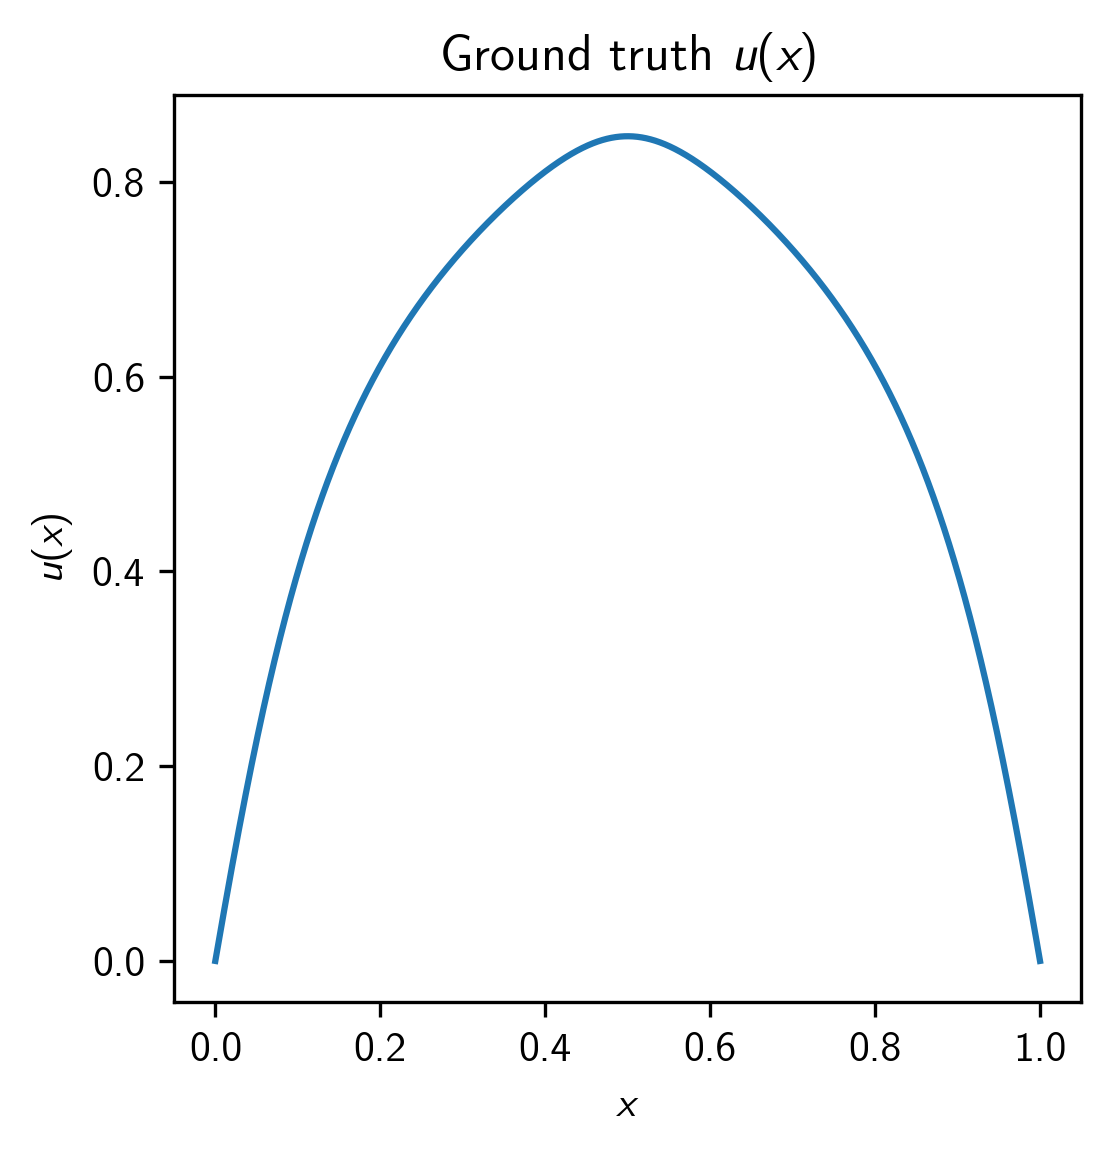
\includegraphics[width=\textwidth]{../Problem_A/GT_u.png} % example-image-a are preinstalled placehoder images
        \caption{Ground truth $u(x)$}
    \end{subfigure}
    %
    \begin{subfigure}[b]{0.3\textwidth}
        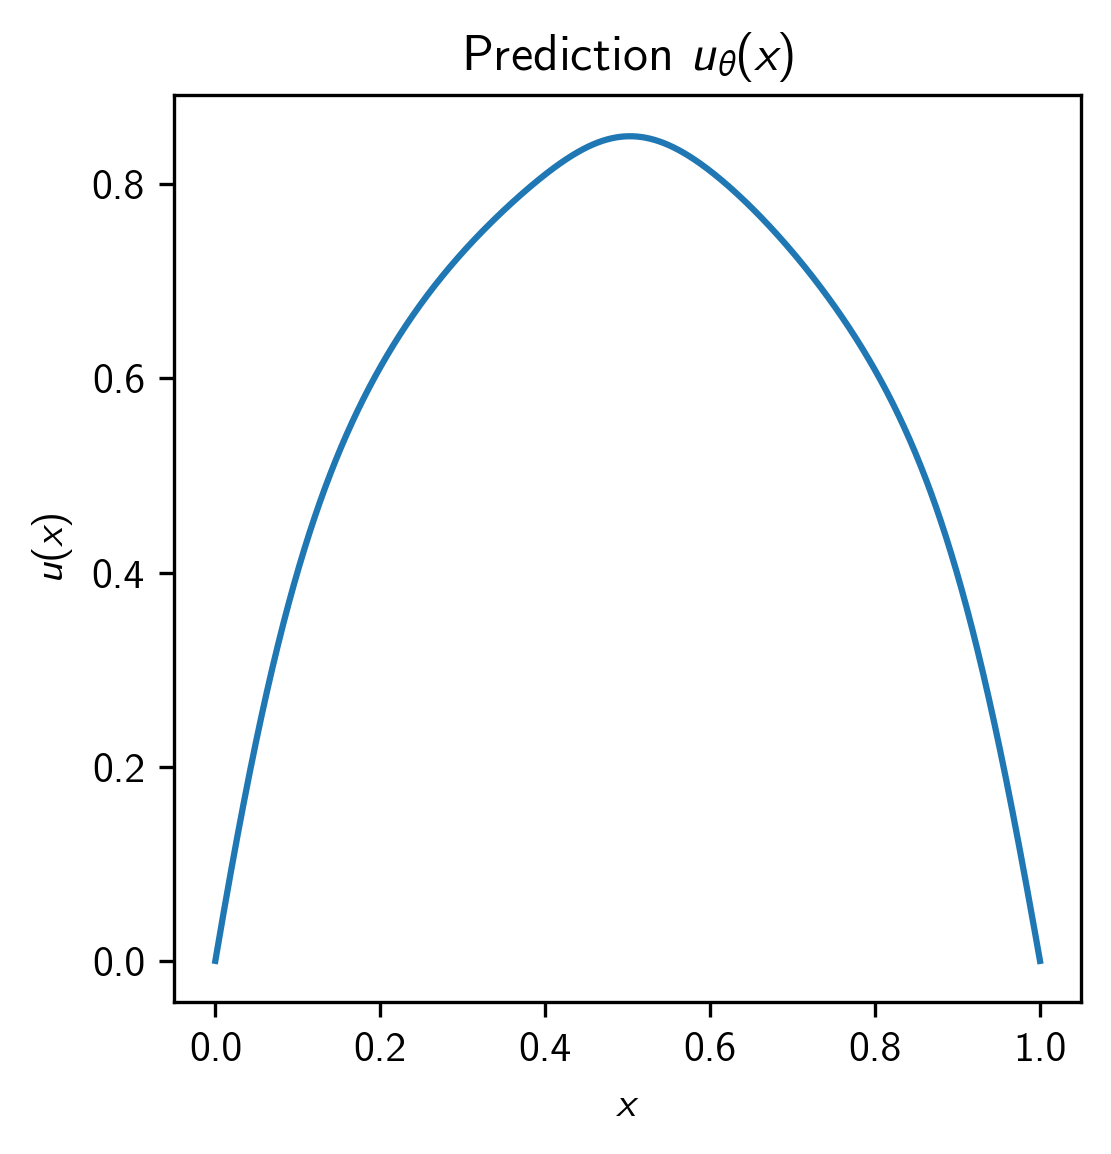
\includegraphics[width=\textwidth]{../Problem_A/predicted_u.png}
        \caption{Prediction $u_\theta(x)$}
    \end{subfigure}
    %
    \begin{subfigure}[b]{0.315\textwidth}
        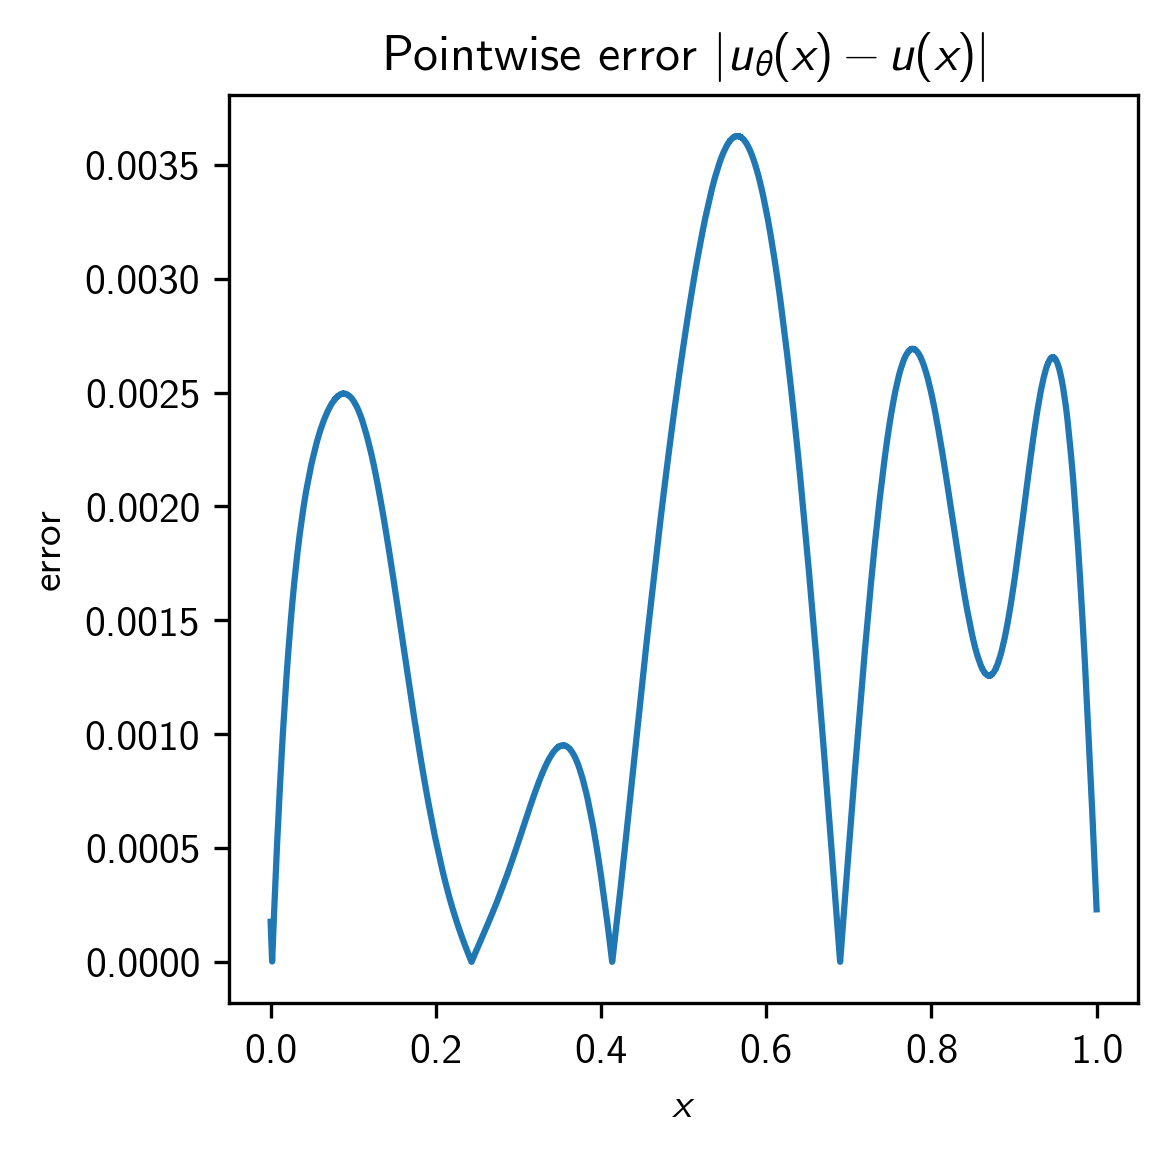
\includegraphics[width=\textwidth]{../Problem_A/pointwise_error_u.png}
        \caption{Pointwise error $|u(x) - u_\theta(x)|$}
    \end{subfigure}
    \caption{Experiment results of MLP for displacement $u(x)$}
    \label{fig:problem_A_u} 
\end{figure}

\begin{figure}[H]
	\centering
	\begin{subfigure}[b]{0.3\textwidth}
		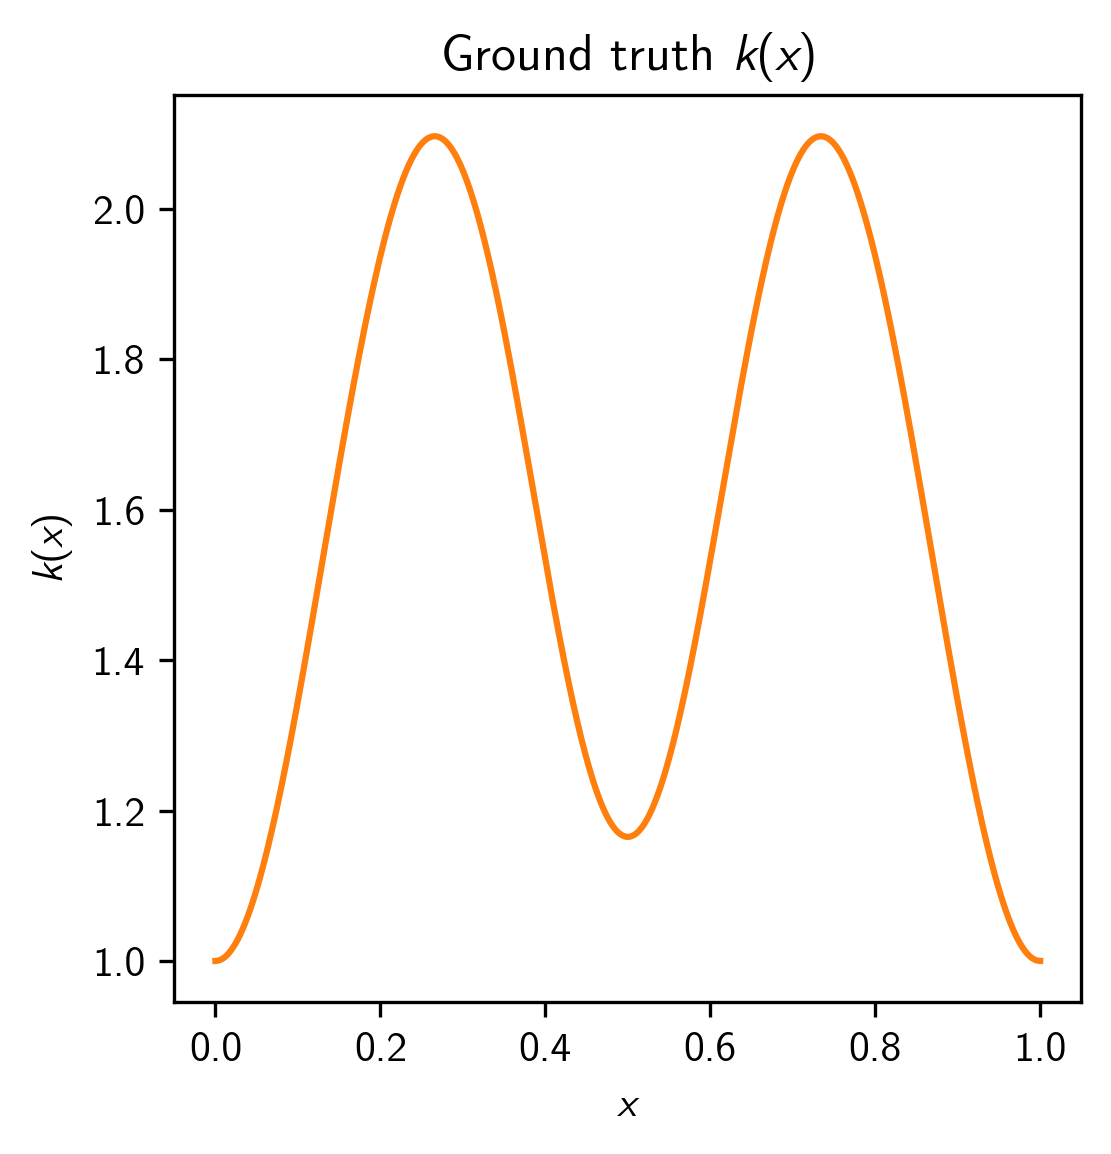
\includegraphics[width=\textwidth]{../Problem_A/GT_k.png} % example-image-a are preinstalled placehoder images
		\caption{Ground truth $k(x)$}
	\end{subfigure}
	%
	\begin{subfigure}[b]{0.3\textwidth}
		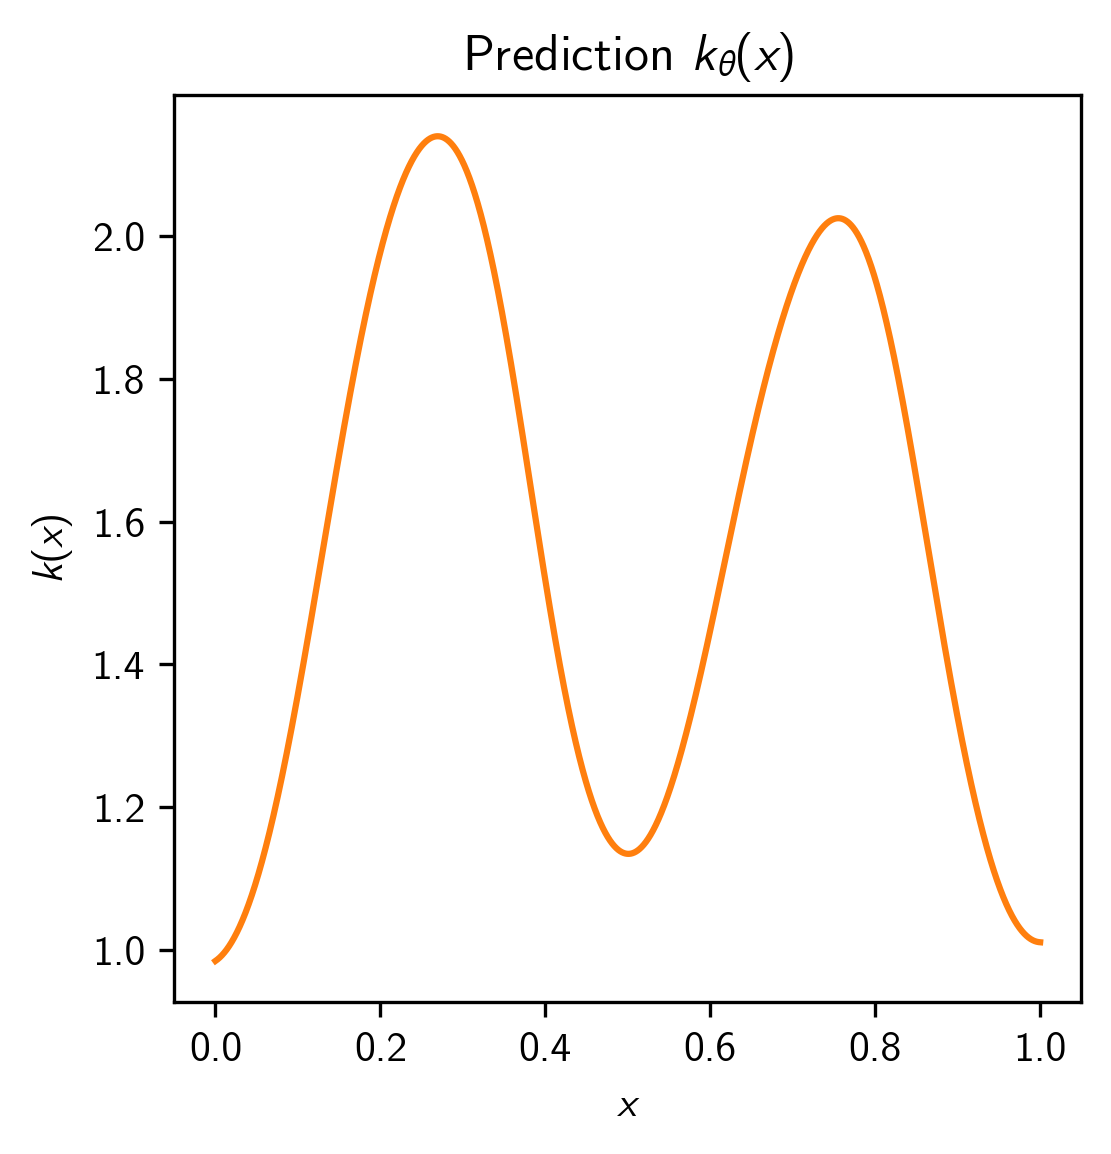
\includegraphics[width=\textwidth]{../Problem_A/predicted_k.png}
		\caption{Prediction $k_\theta(x)$}
	\end{subfigure}
	%
	\begin{subfigure}[b]{0.3\textwidth}
		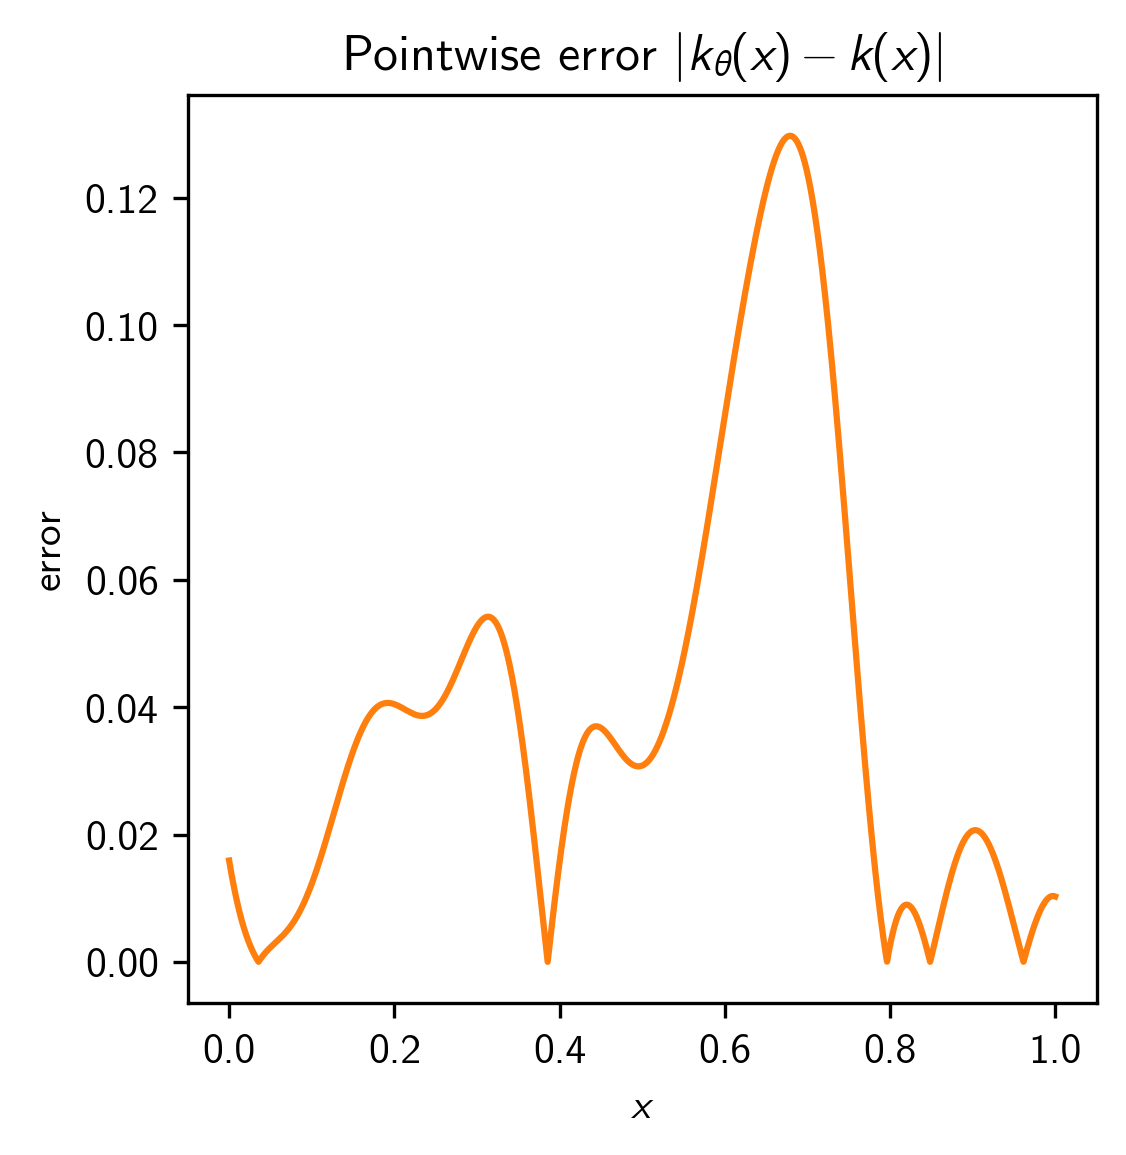
\includegraphics[width=\textwidth]{../Problem_A/pointwise_error_k.png}
		\caption{Pointwise error $|k(x) - k_\theta(x)|$}
	\end{subfigure}
	\caption{Experiment results of MLP for Young's modulus $k(x)$}
	\label{fig:problem_A_k} 
\end{figure}

\begin{figure}[H]
	\centering
	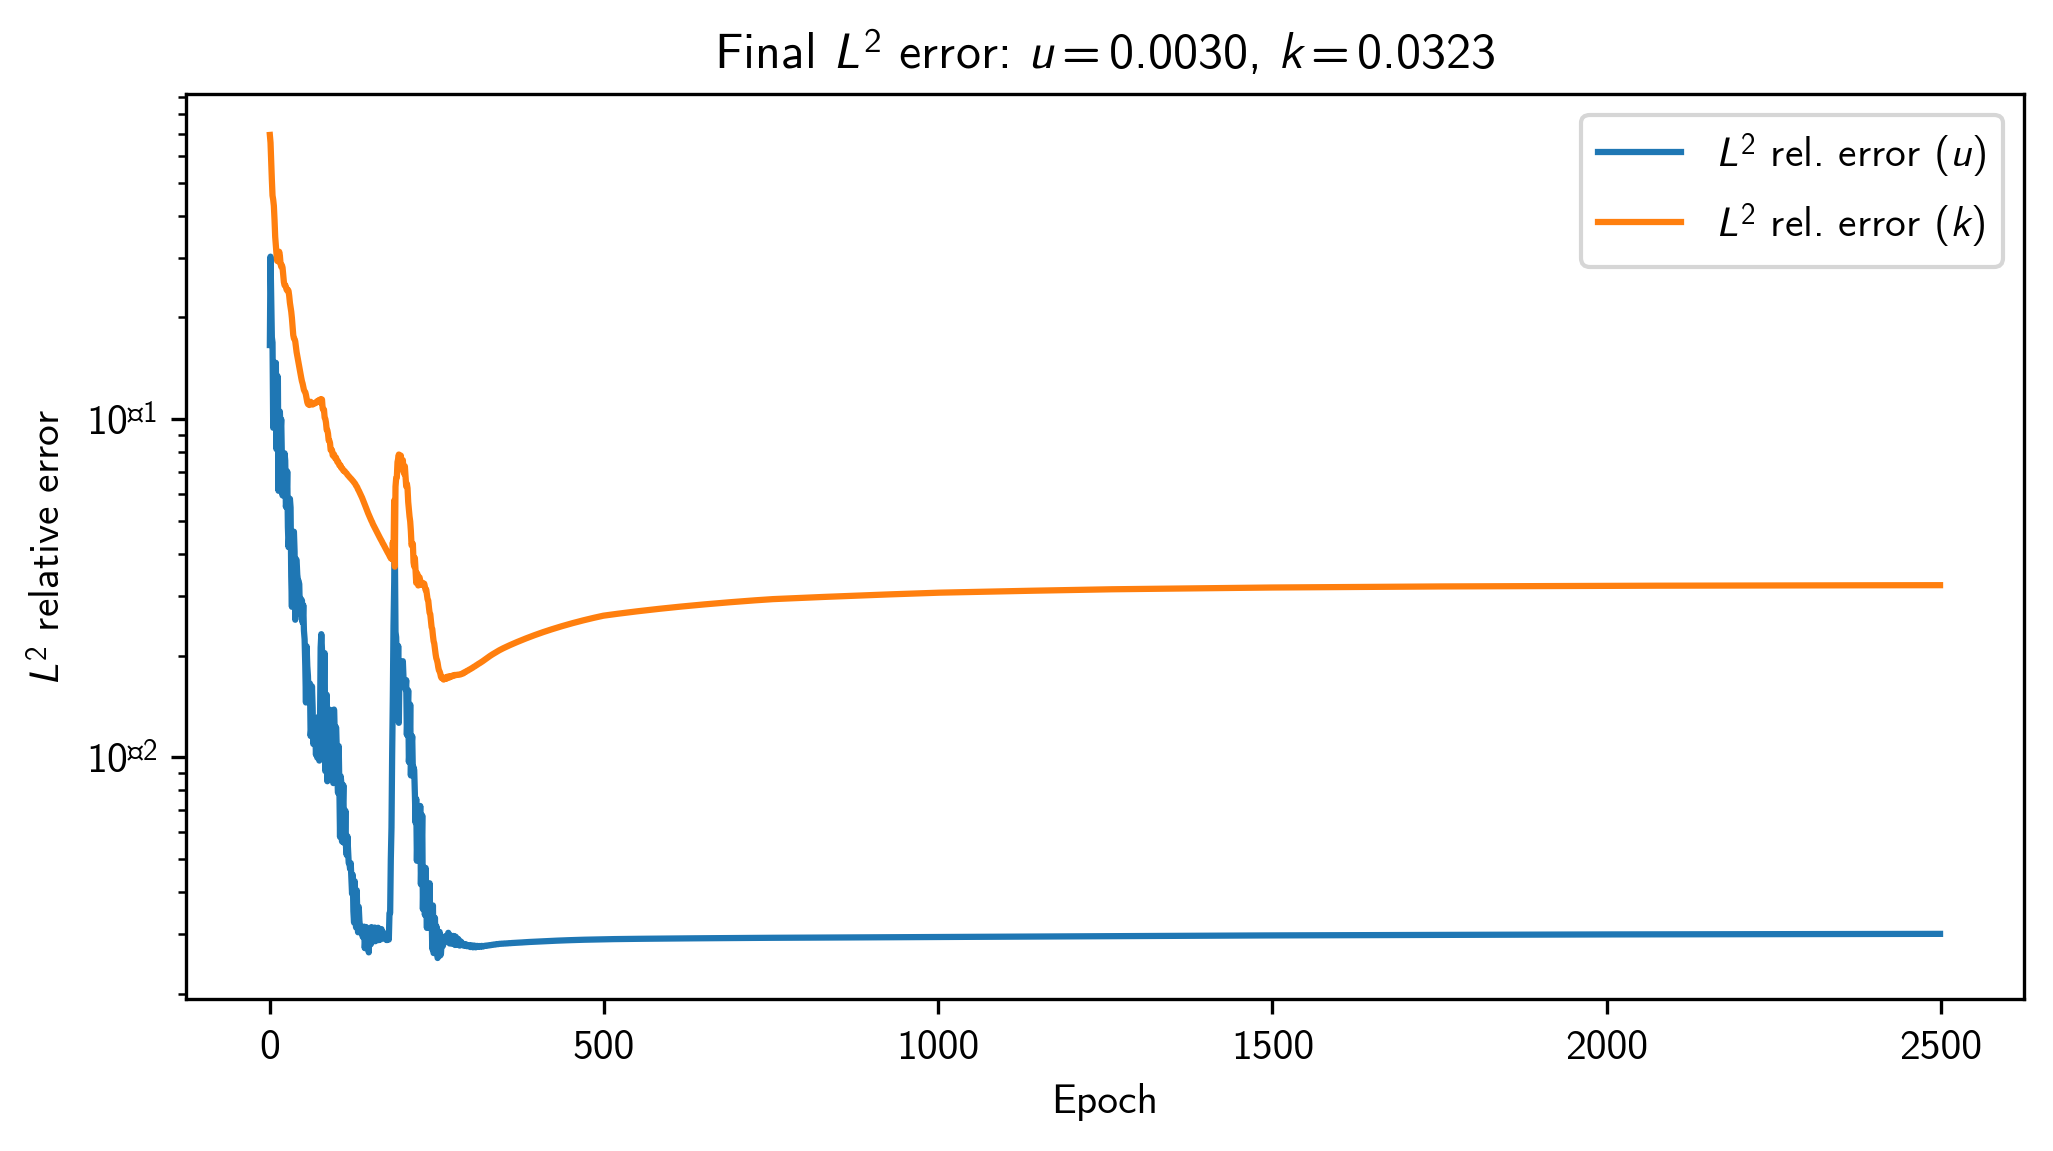
\includegraphics[width=0.8\textwidth]{../Problem_A/error_vs_epoch.png}
	\caption{Evolution of $L^2$ relative error for Problem A}
	\label{fig:problem_A_loss_history} 
\end{figure}


\subsection{Discussion}

As can be seen in Figure \ref{fig:problem_A_u} and Figure \ref{fig:problem_A_k}, the VPINN performs remarkably well, especially on the displacement field $u(x)$. The Young's modulus $k(x)$ is approximated well in terms of the general shape of the function, although some pointwise errors still remain. This was to be expected, since after all the dataset contained labeled (noisy) measurements of $u(x)$, but none of $k(x)$, and it is known that physics-informed models can greatly benefit from labeled data even in small amounts.

As shown in Figure \ref{fig:problem_A_loss_history}, the $L^2$ relative error has clearly been minimized to its full potential, indicating that further training with the same hyperparameters and model architecture would not benefit the performance any further. The final error for $k(x)$ is greater than that of $u(x)$, which makes sense when we visually analyze both their predictions as mentioned before.




%%%%%%%%%%%%%%%%%%%%%%


\chapter{Problem B}
\label{ch:problem_B}
%
\section{Problem Description}

Problem B consists in solving for the pressure field $u(x)$ in a 2-dimensional heterogeneous porous medium. The medium is composed of two distinct material phases with significantly different permeabilities, given by $\mu(x)$ which is provided in the dataset.

\begin{equation}
	\mu(x) =
	\begin{cases}
		\mu_1 = 10, & x\in\Omega_1\quad\text{(high permeability phase)}\\
		\mu_2 = 2, & x\in\Omega_2\quad\text{(low permeability phase)}
	\end{cases}       
\end{equation}

\begin{figure}[H]
	\centering
	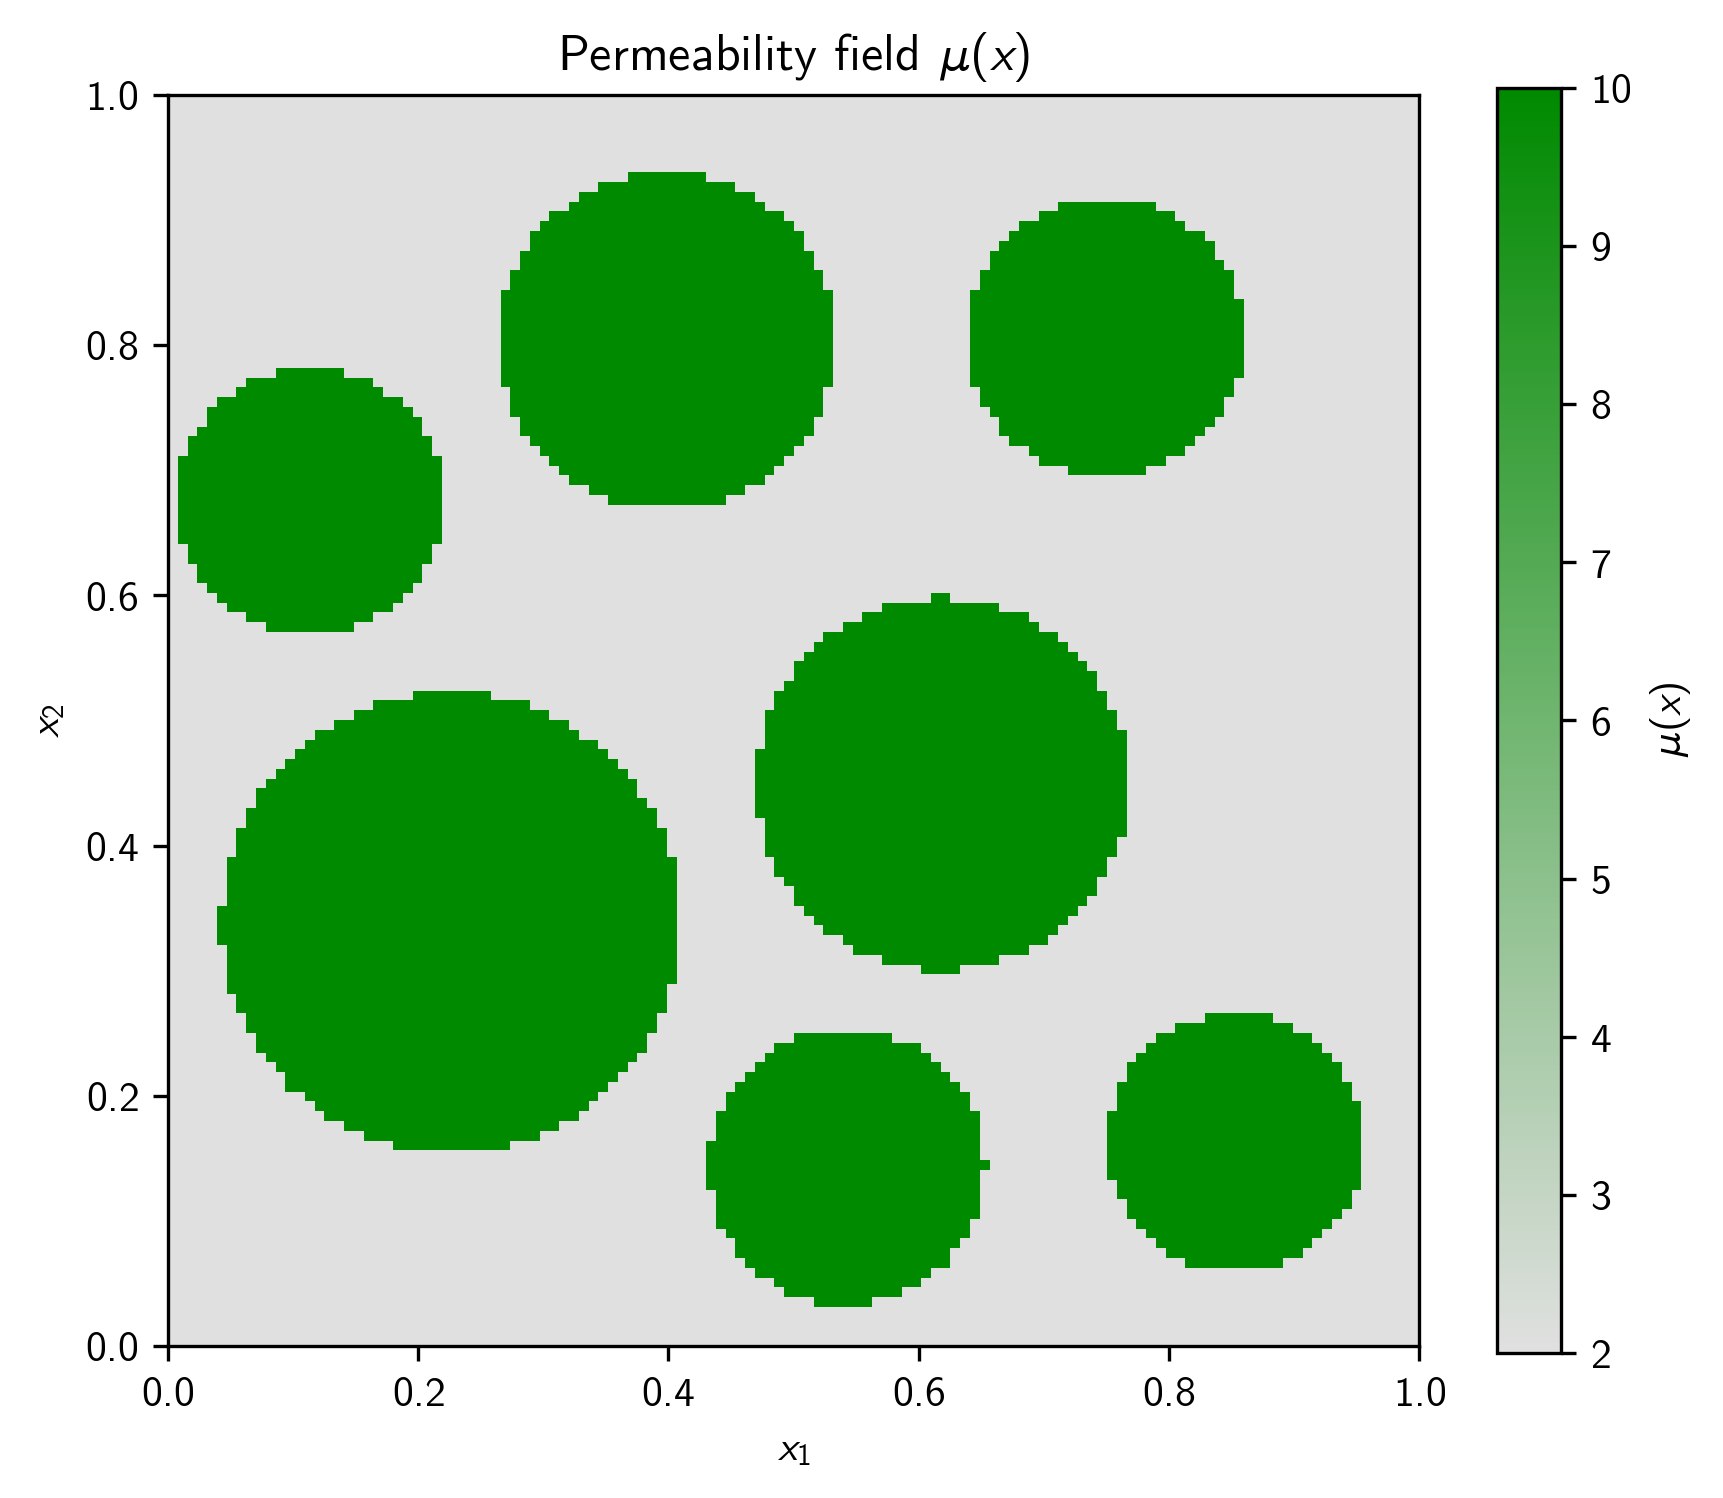
\includegraphics[width=0.7\textwidth]{../Problem_B/mu_field.png}
	\caption{Permeability field $\mu(x)$}
	\label{fig:problem_B_mu_field} 
\end{figure}

The governing PDE for this problem is the Darcy flow equation, namely

\begin{equation}
	-\nabla\cdot \left( \mu(x) \nabla u(x) \right) = f, \quad x\in\Omega = [0, 1]^2
\end{equation}

\noindent
where $f=0$ is the source term (no source or sink in this case) and $\Omega$ is the computational domain containing the sub-domains with different permeabilities $\Omega_1, \Omega_2$.

The PDE is subject to the following boundary conditions $g_D(x)$:

\begin{equation}
	g_D(x) =
	\begin{cases}
		1, & x_1 = 0\\
		0, & x_1 = 1\\
		\text{linear interpolation}, & x_2 = 0 \text{ or } 1
	\end{cases}       
\end{equation}



\section{Methodology}
%
\subsection{The method selection}
%Describe the method you use and the reason for choosing it.
%

The method of choice for this problem is to use a ParticleWNN approach. The reason for this choice is that this method applicable to forward problems (like Problem B) and performs well on low dimensional data. Since we are learning the solution for a single material field, a DNO is not necessary for this problem. ParticleWNN chosen over other weak-form methods due to its ability to handle sharp gradients and locally complex solutions. This is suitable for the specific dataset at hand, given that the material field $\mu(x)$ has instantaneous changes in permeability rather than smooth transitions, as can be seen in Figure \ref{fig:problem_B_mu_field}.

\subsection{The loss function}
%Describe the loss function you use and the corresponding hyperparameters (i.e., loss weights, collocation points/integral points, and so on) used in training.
%

The loss function used in this problem comprises 2 terms: a boundary condition loss and a PDE loss. The boundary condition loss is defined as the Mean Squared Error (MSE) between the predicted pressure $u_\theta(x)$ at the boundary and the true boundary pressure $g_D(x)$:

\begin{equation}
	\mathcal{L}_\mathrm{bd} = \frac{1}{\left| \partial\Omega \right|} \sum_{x\in\partial\Omega}^{} \left| u_\theta (x) - g_D(x) \right|^2
\end{equation}

\noindent
where $\partial\Omega$ is the boundary of the computational domain.

To compute the PDE loss, we first compute the weak residuals $R_n$ of each test function $v_n(x)$. The test functions used in this case are Wendland Compactly Supported Radial Basis Functions (CSRBFs). The centers of said CSRBFs are found by fisrt sampling $N_c = 10^4$ "particles" uniformly inside the computational domain, then every training epoch taking a random subset of them for the computation of the weak residuals. The residuals are approximated by Gauss-Legendre quadrature, as follows:

\begin{align}
	R_n &= \int_{\Omega} \left( \mu(x) \nabla u_\theta(x) \nabla v_n(x) - f(x) v_n(x) \right) dx \\
	&\approx \sum_{j=1}^{N_\mathrm{int}} \left( \mu (x_j) \nabla u_\theta(x_j) \nabla v_n(x_j) - f(x_j) v_n(x_j) \right) w_j
\end{align}

\noindent
where $N_\mathrm{int}$ is the number of integral points to use in the quadrature, chosen here to be $N_\mathrm{int} = 15$, and $w_j$ are the quadrature weights. The permeability field $\mu(x)$ is only defined at discrete grid locations (provided by the dataset), however it must be evaluated at quadrature points for the calculation of the $R_n$. To do this, bilinear interpolation between the grid points is used.

\newpage
The PDE loss is then given by

\begin{align}
	\mathcal{L}_\mathrm{PDE} &= \frac{1}{N_\mathrm{test}} \sum_{i=1}^{N_\mathrm{test}} R_i^2
\end{align}

The number of test functions $N_\mathrm{test}$ is chosen here to be $N_\mathrm{test} = 200$.

The total training loss $\mathcal{L}_\theta$ is computed as a weighted sum of the 2 losses mentioned previously, where the weights associated to each loss are hyperparameters.

\begin{equation}
	\mathcal{L}_\theta = w_\mathrm{bd} \mathcal{L}_\mathrm{bd} + w_\mathrm{PDE} \mathcal{L}_\mathrm{PDE}
\end{equation}






\subsection{The network structure}
%Describe the network structure that you use during training. 
%

The network structure used for Problem B consists of one MLP with fully connected layers. The network architecture of said MLP can be found in Table \ref{tab:problem_B_network}.


\begin{table}[H]
	\centering
	\caption{Network architecture of ParticleWNN for Problem B}
	\label{tab:problem_B_network}
	\begin{tabular}{llll}
		\hline
		\textbf{Layer} & \textbf{Size / Neurons} & \textbf{Activation Function} & \textbf{Notes} \\
		\hline
		Input Layer        & 2                                & $\sigma_B(x)$         & - \\
		Hidden Layer 1     & 200                              & $\sigma_B(x)$       & Fully connected \\
		Hidden Layer 2     & 50                               & $\sigma_B(x)$       & Fully connected \\
		Hidden Layer 3     & 50                               & $\sigma_B(x)$       & Fully connected \\
		Hidden Layer 4       & 100                            & $\sigma_B(x)$    & Fully connected \\
		Output Layer       & 1                              & Linear       & - \\
		\hline
	\end{tabular}
\end{table}

The custom activation function $\sigma_B(x)$ used for all layers except the output layer is

\begin{equation}
	\sigma_B(x) = \sin(\pi x + \pi) + \sin(x)
\end{equation}

\noindent
which identical to the activation used for the hidden layers in Problem A, as seen in equation (\ref{eq:custom_activation}). Once again the same reasoning is applied: the sinusoidal activation is used to try to capture fine details \cite{sitzmann2020implicitneuralrepresentationsperiodic}. Other common activations including Sigmoid, Tanh or ReLU were also tried in this problem, but this custom activation yielded the best performance.

The Linear activation of the output layer ensures that $u_\theta(x)$ can be both greater and smaller than 0.


\subsection{The code link}
{\color{blue}Please provide the hyperlink (e.g., GitHub, Google Colab, or Kaggle Notebook) to your original code for solving this problem.} 
%


\newpage
\section{Numerical Results}
%
\subsection{Experiment Setups}
%Describe the experiment setups for training the model.
%

The hyperparameters used in the experimental setup are listed in Table \ref{tab:training_setup_B}. 


\begin{table}[H]
	\centering
	\caption{Numerical setup for training the ParticleWNN in PyTorch}
	\label{tab:training_setup_B}
	\begin{tabular}{ll}
		\hline
		\textbf{Parameter} & \textbf{Value} \\
		\hline
		$w_\mathrm{bd}$     & $1\times10^6$ \\
		$w_\mathrm{PDE}$    & 1 \\
		Optimizer           & Adam \\
		Learning Rate (initial)       & $1 \times 10^{-2}$ \\
		Batch Size          & 200 \\
		Number of Epochs    & 60 \\
		Learning Rate Scheduler & StepLR \\
		Decay Rate ($\alpha$/N epochs) &  0.9/3\\
		Hardware            & NVIDIA RTX 3050 Laptop (4GB) \\
		Precision           & Float32 \\
		Early Stopping      & No \\
		\hline
	\end{tabular}
\end{table}

\subsection{Numerical Results}
%Report the results (e.g., the time consumption and the $L^2$ relative error) you obtained in this section.

The results of the experiment are shown in Figure \ref{fig:problem_B_u}. The loss history is shown in Figure \ref{fig:problem_B_loss_history}.
%
\begin{figure}[H]
	\centering
	\begin{subfigure}[b]{0.325\textwidth}
		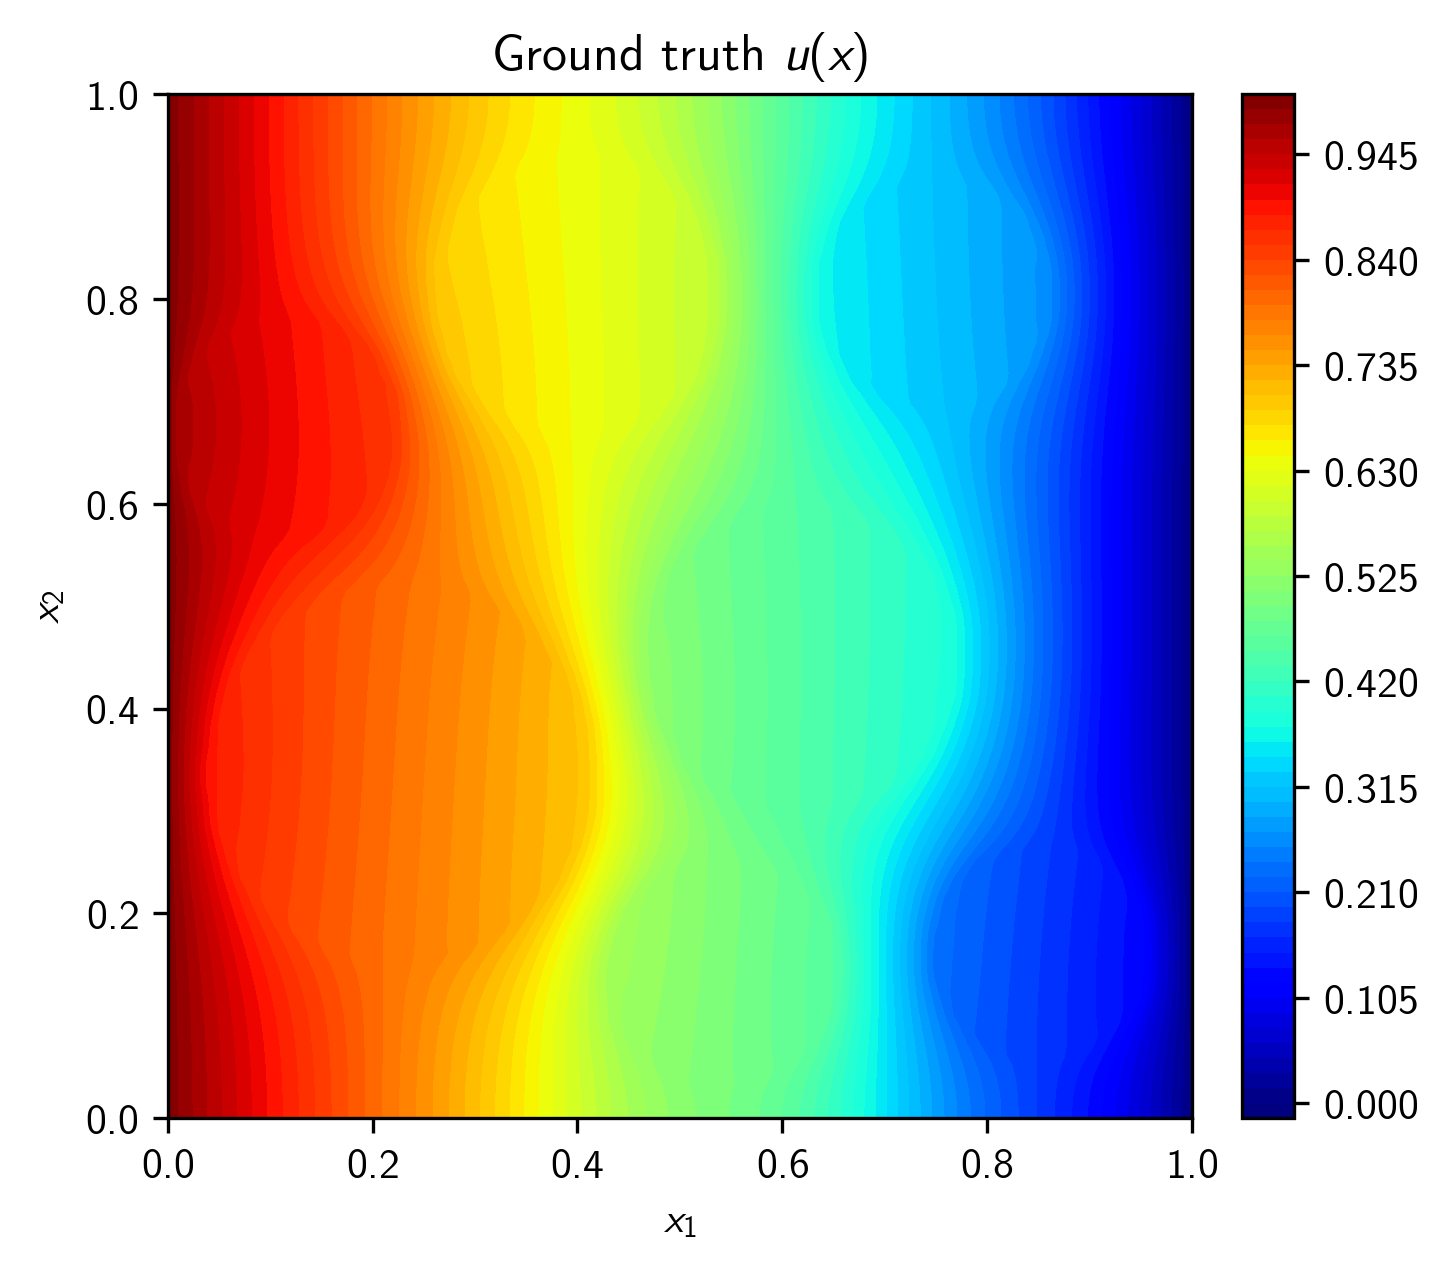
\includegraphics[width=\textwidth]{../Problem_B/GT_u.png} % example-image-a are preinstalled placehoder images
		\caption{Ground truth $u(x)$}
	\end{subfigure}
	%
	\begin{subfigure}[b]{0.325\textwidth}
		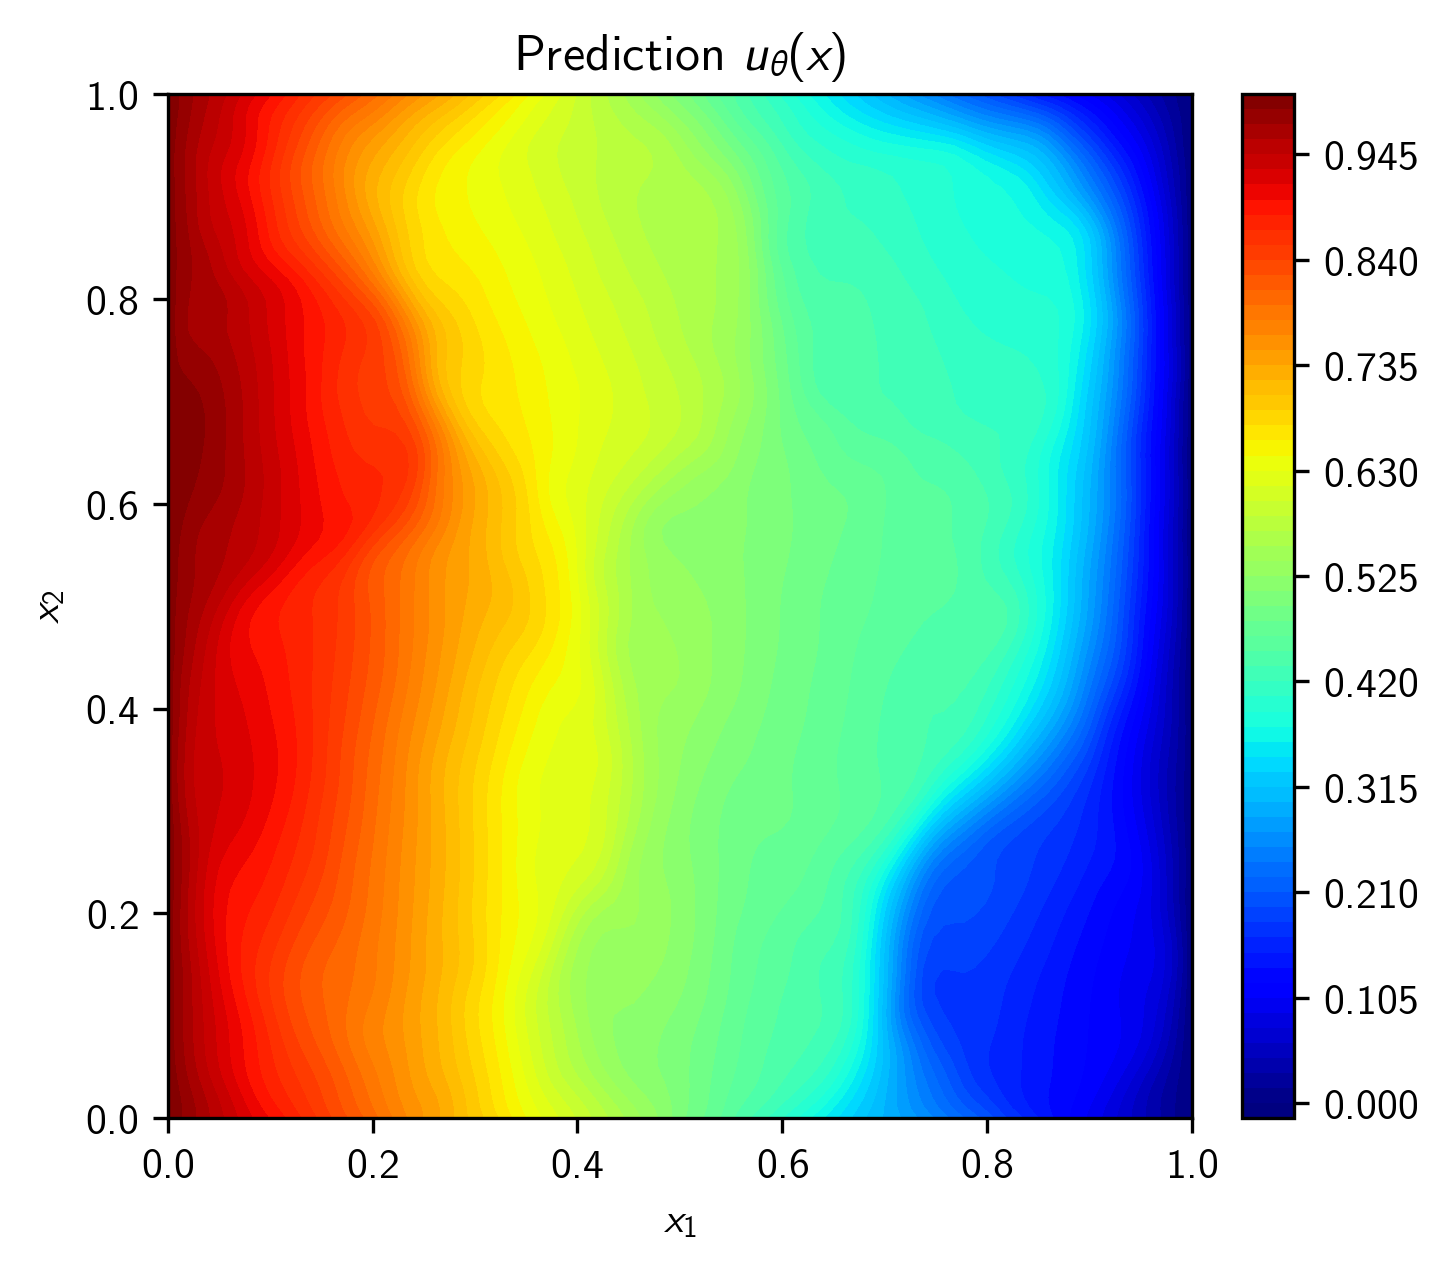
\includegraphics[width=\textwidth]{../Problem_B/predicted_u.png}
		\caption{Prediction $u_\theta(x)$}
	\end{subfigure}
	%
	\begin{subfigure}[b]{0.325\textwidth}
		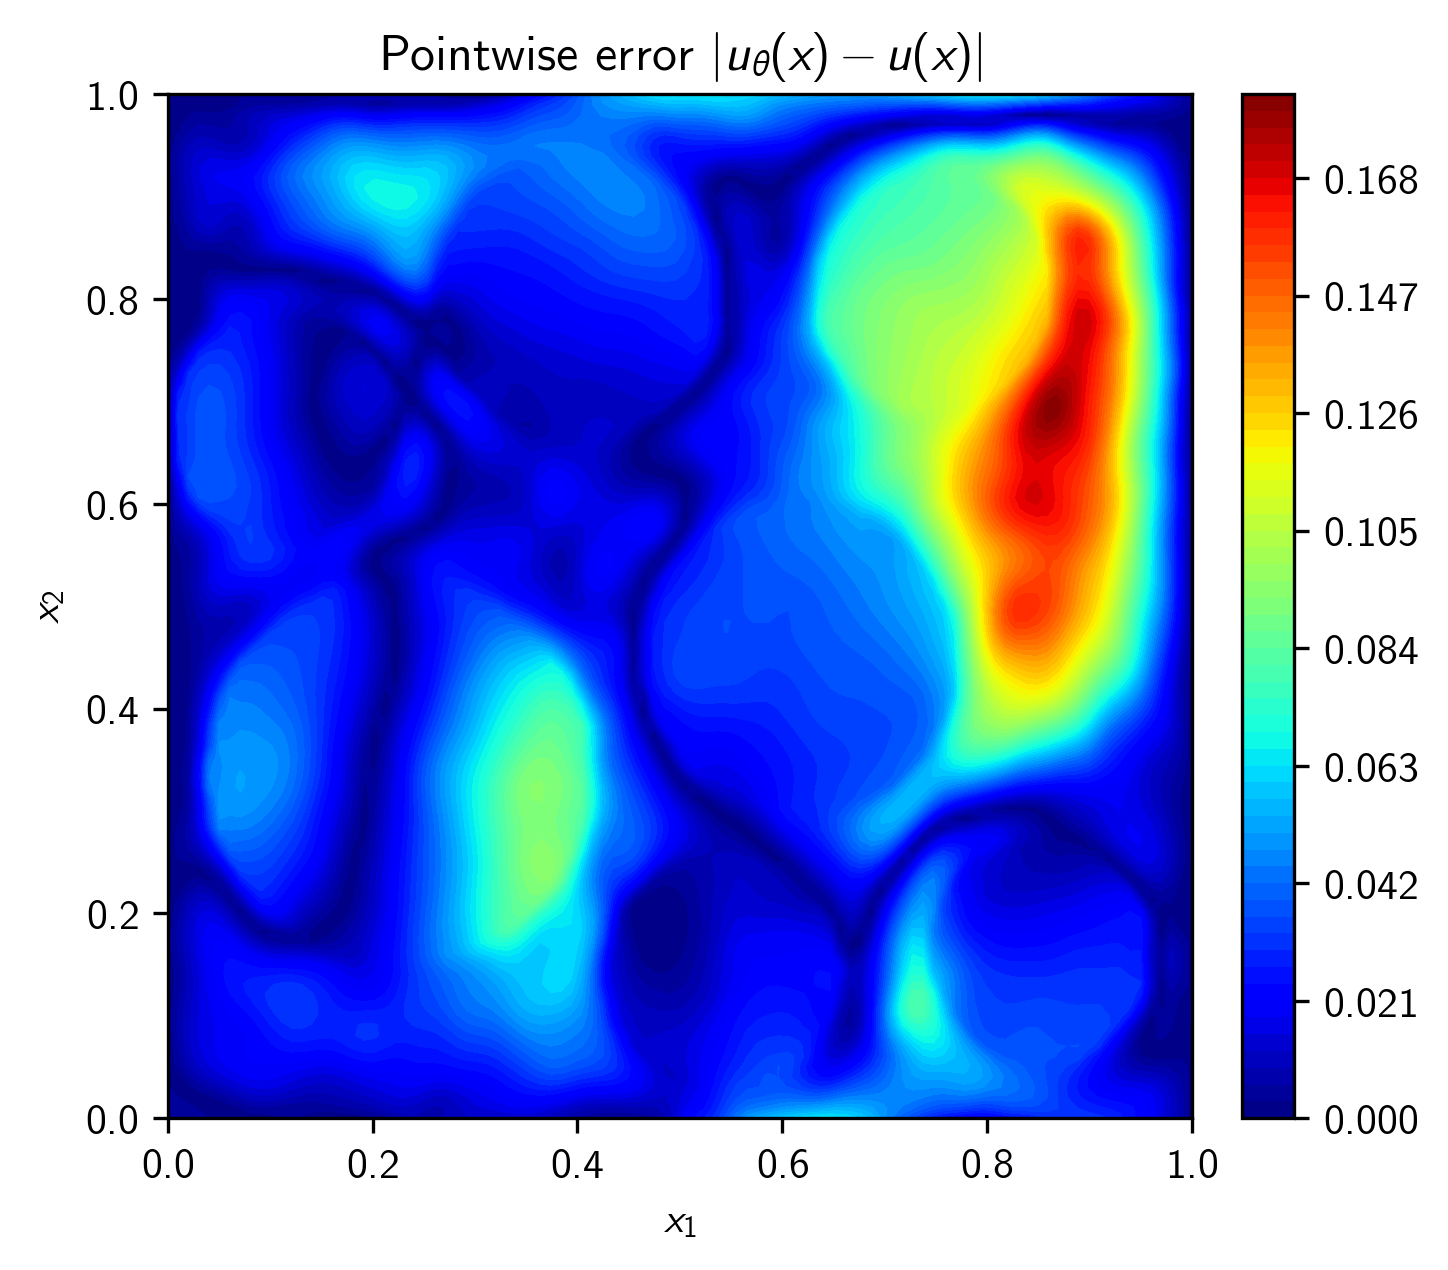
\includegraphics[width=\textwidth]{../Problem_B/pointwise_error_u.png}
		\caption{Pointwise error $|u(x) - u_\theta(x)|$}
	\end{subfigure}
	\caption{Experiment results of Problem B}
	\label{fig:problem_B_u} 
\end{figure}

\begin{figure}[H]
	\centering
	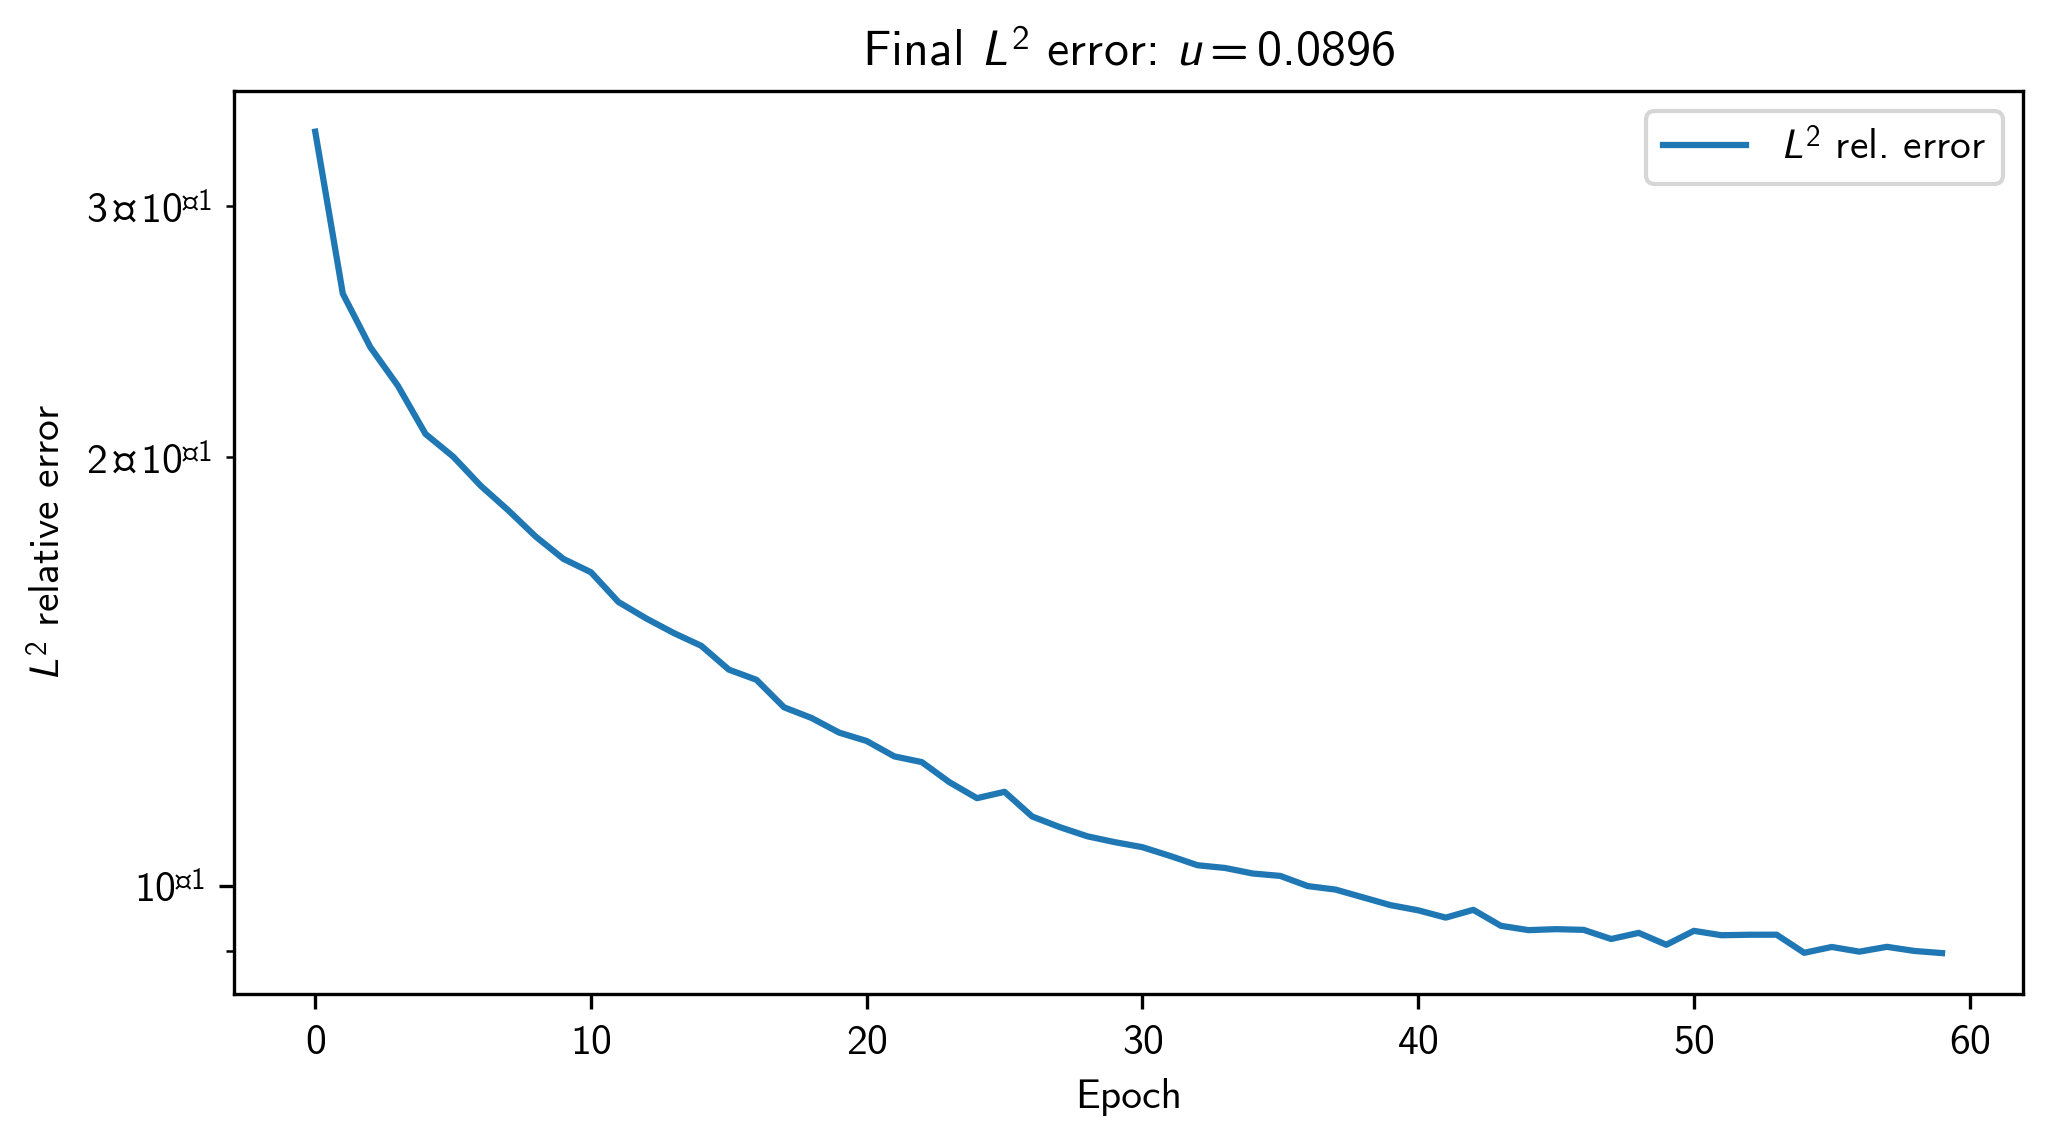
\includegraphics[width=0.8\textwidth]{../Problem_B/error_vs_epoch.png}
	\caption{Evolution of $L^2$ relative error for Problem B}
	\label{fig:problem_B_loss_history} 
\end{figure}



\subsection{Discussion}

As can be seen in Figure \ref{fig:problem_B_u}, the ParticleWNN is able to capture the general shape of the pressure field, but it struggles to capture the finer details. This could possibly be due to the number of parameters in the network being too small, or simply an incorrect choice of hyperparameters. Nevertheless, the boundary conditions are well respected.

Looking at the $L^2$ relative error in Figure \ref{fig:problem_B_loss_history}, we can see that it decreases monotonically and smoothly, implying that good learning parameters have been found. The curve flattens out towards the end, which means that training the model for more epochs will not yield a significant increase in performance with the current set of hyperparameters.





%%%%%%%%%%%%%%%%%%%%%%
\chapter{Problem C}
\label{ch:problem_C}
%
\section{Problem Description}
%

Problem C consists in learning the solution operator that maps a thermal conductivity field $a(x, y)$ to a temperature field $u(x, y)$ in a heterogeneous solid material. The PDE governing this system is

\begin{equation}
	-\nabla\cdot\left( a(x,y)\nabla u(x, y) \right) = f, \quad (x,y)\in\Omega = [0,1]^2 
\end{equation}

\noindent
where $f = 10$ is a uniform heat source and $\Omega$ is the computational domain.
The PDE must satisfy a constant temperature of 0 at the boundary $\partial\Omega$ of the computational domain, as expressed by the following boundary condition:

\begin{equation}
	u(x,y) = 0, \quad (x,y)\in\partial\Omega
\end{equation}

The provided dataset contains 1000 labeled pairs of conductivity fields $a(x,y)$ and temperature fields $u(x,y)$.

\section{Methodology}
%
\subsection{The method selection}
%Describe the method you use and the reason for choosing it.
%

Since this problem involves learning a mapping from an arbitrary material field to a solution field, an operator is needed. Given that the dataset at hand is fully labeled, using a physics-informed DNO approach is not considered necessary in this case, as the network may learn the mapping completely through minimization of the data loss.

A visual analysis of the dataset for $a(x,y)$ shows that the material fields contain periodically-varying structures, as can be seen in Figure \ref{fig:problem_C_input_field}. This makes the Fourier Neural Operator (FNO) an excellent choice for this type of problem, as it can naturally learn the main frequency components in material and solution fields. Additionally, the FNO is computationally efficient, as it outputs a full solution field per forward pass, rather than a single point like DeepONet.


\begin{figure}[H]
	\centering
	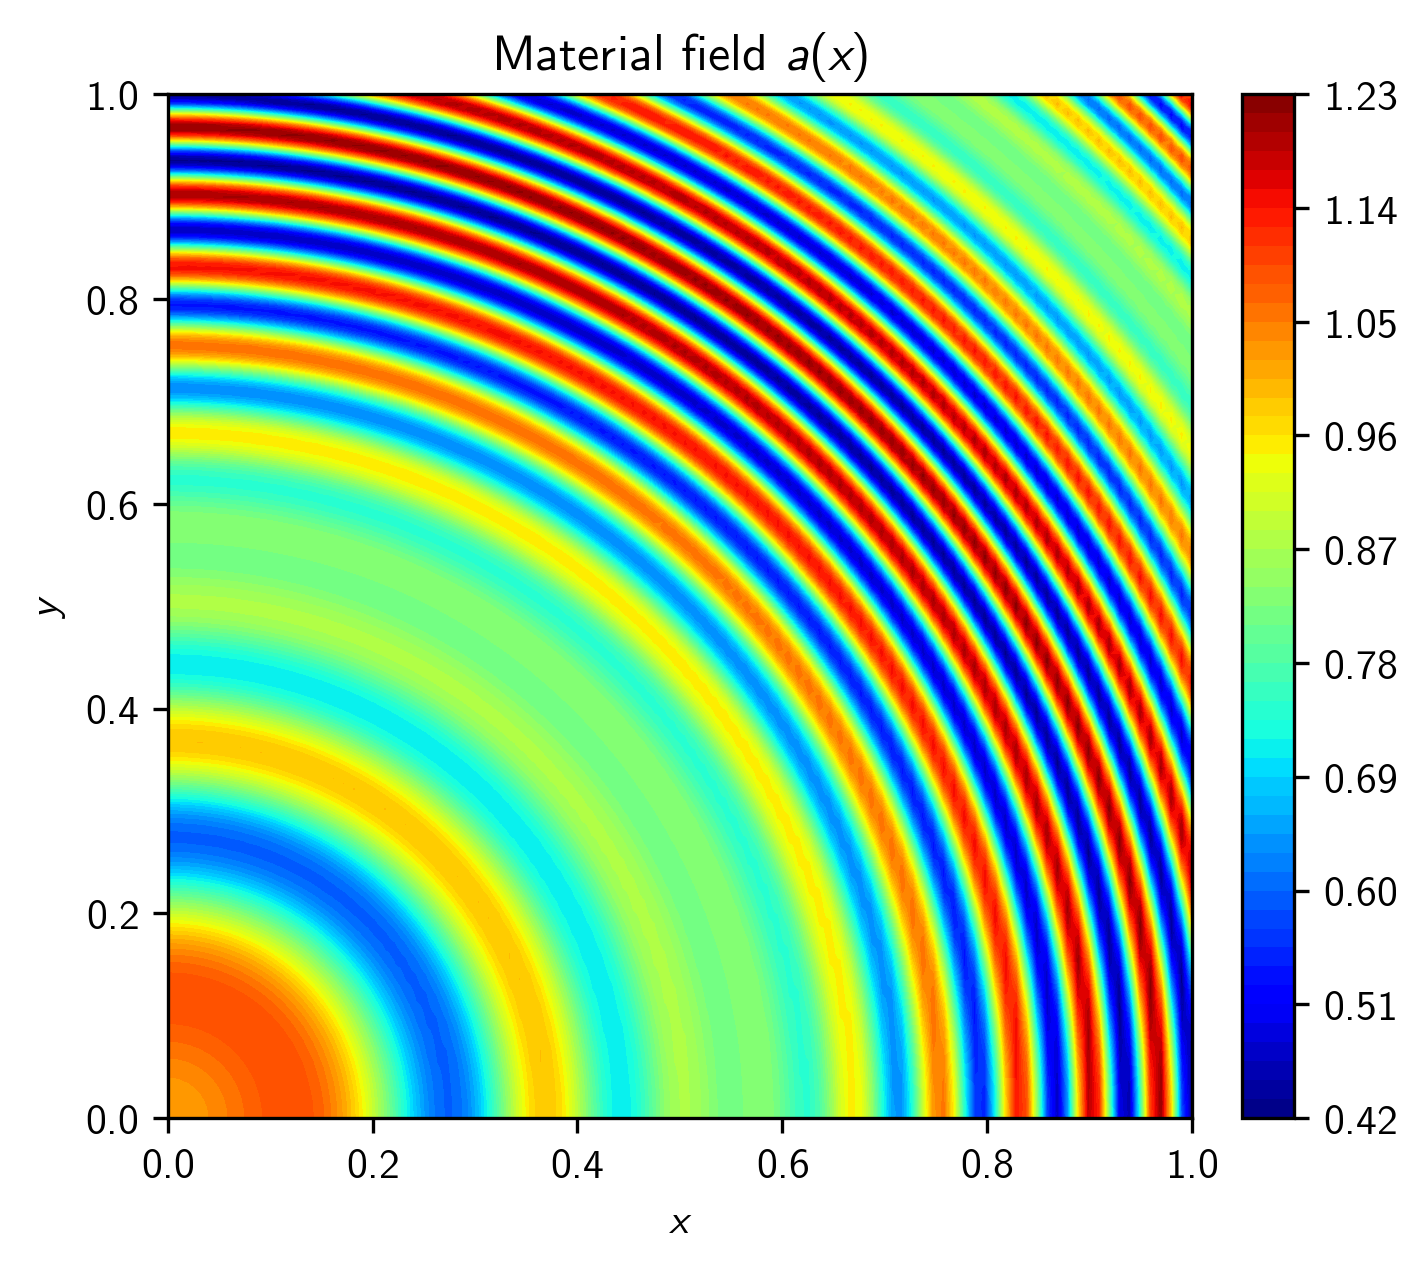
\includegraphics[width=0.7\textwidth]{../Problem_C/input_a.png}
	\caption{Example conductivity field $a(x,y)$}
	\label{fig:problem_C_input_field} 
\end{figure}

\subsection{The loss function}
%Describe the loss function you use and the corresponding hyperparameters (i.e., loss weights, collocation points/integral points, and so on) used in training.
%

The loss function for this problem is remarkably simple, given that no physics-enforcing loss terms are used. Thus, only a data loss is used to compare the prediction of the operator to the ground truth solution field. The total loss is given by

\begin{equation}
	\mathcal{L}_\theta = \frac{1}{N} \sum_{i=1}^{N} \left\Vert \mathcal{G}_\theta \left(a_i(x,y)\right) - u_i(x,y) \right\Vert_2
\end{equation}

\noindent
where $N=1000$ is the number of training examples and $\mathcal{G}_\theta$ is the operator that maps the material field to the solution field: $\mathcal{G}_\theta : a(x,y) \mapsto u_\theta(x,y)$.



\subsection{The network structure}
%Describe the network structure that you use during training. 
%

The network structure used for Problem C is best described by Figure \ref{fig:problem_C_architecture}. As can be seen in the figure, the material field $a(x,y)$ is first "lifted" onto a higher dimensional space by a MLP with Linear activations, before being passed onto the Fourier layers, which perform the following operation:

\begin{equation}
	v_{l+1} = \sigma_C \left[ \mathcal{F}^{-1} \left( R_l \cdot \mathcal{F}(v_l) \right) (x) + W_l v_l(x)\right]
\end{equation}

\noindent
where $v_l$ is the input to layer $l$, $\sigma_C$ is an activation function, $\mathcal{F}$ denotes the Fourier transform, $R_l$ is a tensor of learnable parameters and $W_l$ is a tensor of learnable weights called the "bypass".

After the Fourier layers, the field is projected back to its final dimension by another MLP. This MLP consists of 3 layers, which temporarily change the channel dimension of the field from 40 to 128, then from 128 to 1, as can be seen in Figure \ref{fig:problem_C_architecture}. The activations for the 3 layers in this MLP are Linear, ReLu and Linear, respectively.

The specific parameters of each layer in the network can be found in Table \ref{tab:problem_C_network}.


\begin{figure}[H]
	\centering
	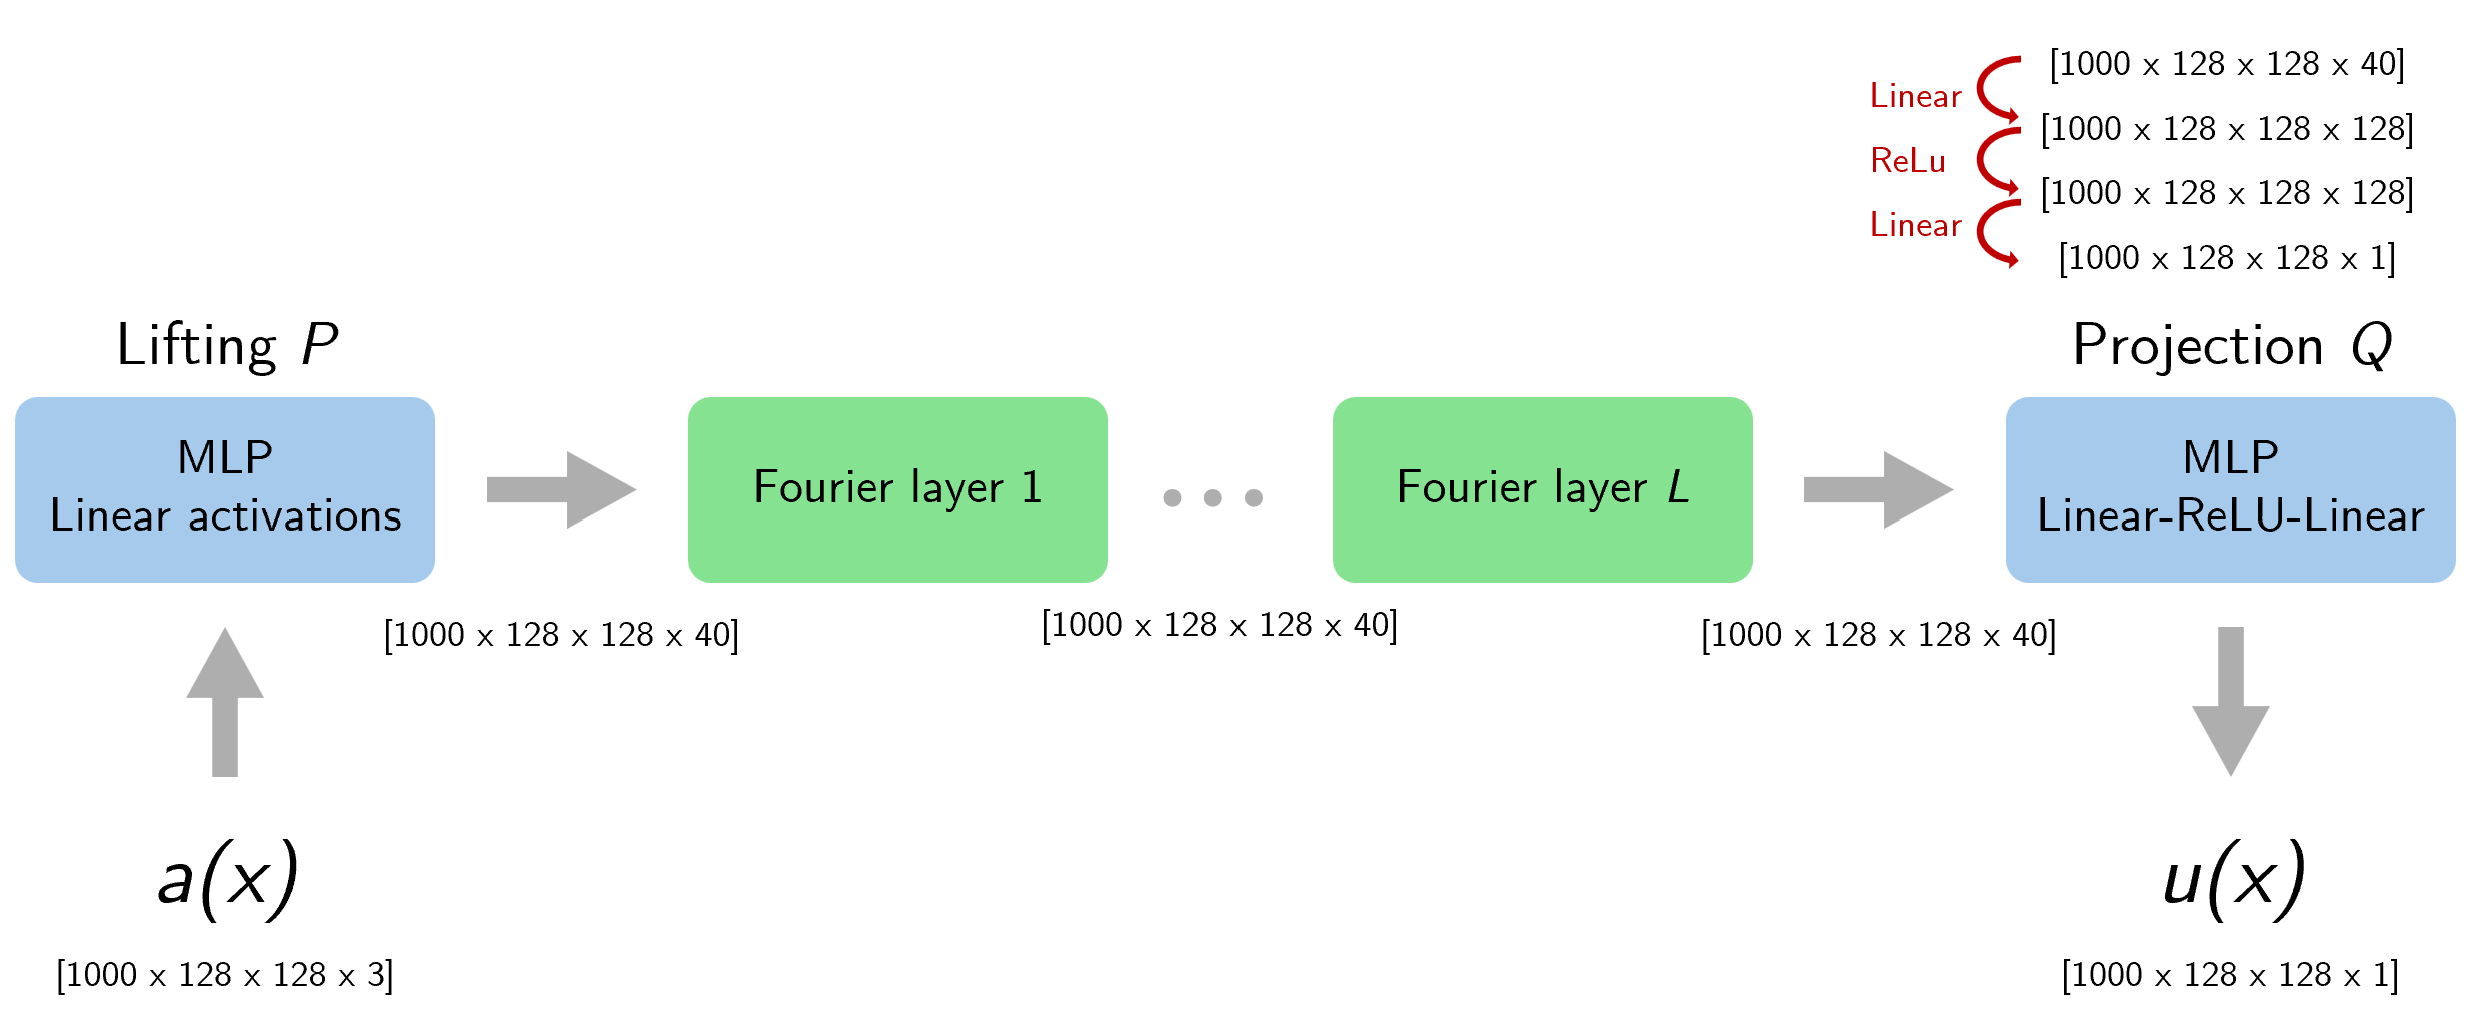
\includegraphics[width=1\textwidth]{../Problem_C/Problem_C_architecture.png}
	\caption{FNO structure for Problem C}
	\label{fig:problem_C_architecture} 
\end{figure}


\begin{table}[H]
	\centering
	\caption{Network architecture of FNO for Problem C}
	\label{tab:problem_C_network}
	\begin{tabular}{llll}
		\hline
		\textbf{Layer} & \textbf{Size / Neurons} & \textbf{Activation Function} & \textbf{Notes} \\
		\hline
		Lifting Layer        & 40                                & Linear         & - \\
		Fourier Layer 1        & 40                                & $\sigma_C(x)$ = ReLU         & 16 modes used \\
		Fourier Layer 2     & 40                              & $\sigma_C(x)$ = ReLU       & 16 modes used \\
		Projection Layer 1     & 128                              & Linear       & - \\
		Projection Layer 2     & 128                              & ReLU       & - \\
		Projection Layer 2     & 1                              & Linear       & - \\
		\hline
	\end{tabular}
\end{table}

\subsection{The code link}
{\color{blue}Please provide the hyperlink (e.g., GitHub, Google Colab, or Kaggle Notebook) to your original code for solving this problem.} 
%
\section{Numerical Results}
%
\subsection{Experiment Setups}
%Describe the experiment setups for training the model.
%

The hyperparameters used in the experimental setup are listed in Table \ref{tab:training_setup_C}. 


\begin{table}[H]
	\centering
	\caption{Numerical setup for training the FNO in PyTorch}
	\label{tab:training_setup_C}
	\begin{tabular}{ll}
		\hline
		\textbf{Parameter} & \textbf{Value} \\
		\hline
		Optimizer           & Adam \\
		Learning Rate (initial)       & $1 \times 10^{-3}$ \\
		Weight Decay       & $1 \times 10^{-3}$ \\
		Batch Size          & 5 \\
		Number of Epochs    & 30 \\
		Learning Rate Scheduler & StepLR \\
		Decay Rate ($\alpha$/N epochs) &  0.5/7\\
		Hardware            & NVIDIA RTX 3050 Laptop (4GB) \\
		Precision           & Float32 \\
		Early Stopping      & No \\
		\hline
	\end{tabular}
\end{table}

\subsection{Numerical Results}
%Report the results (e.g., the time consumption and the $L^2$ relative error) you obtained in this section.

\begin{figure}[H]
	\centering
	\begin{subfigure}[b]{0.495\textwidth}
		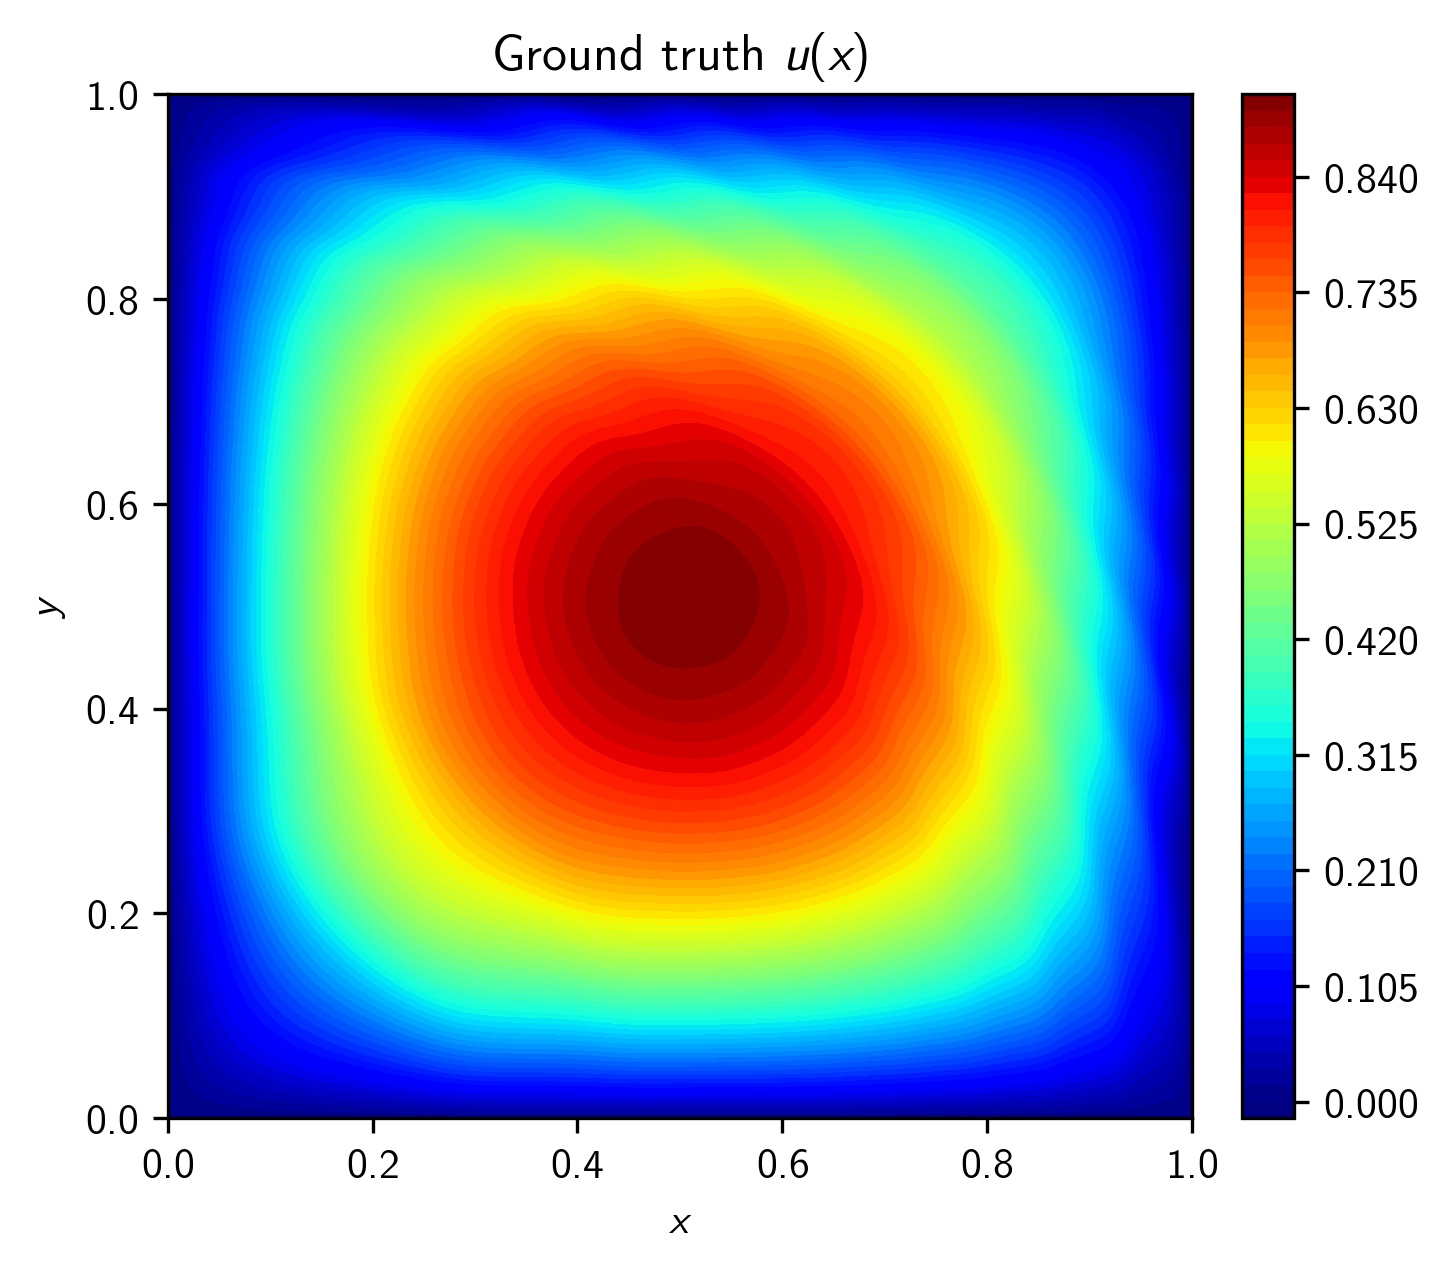
\includegraphics[width=\textwidth]{../Problem_C/GT_u.png}
		\caption{Ground truth $u(x,y)$}
	\end{subfigure}
	\hfill
	\begin{subfigure}[b]{0.495\textwidth}
		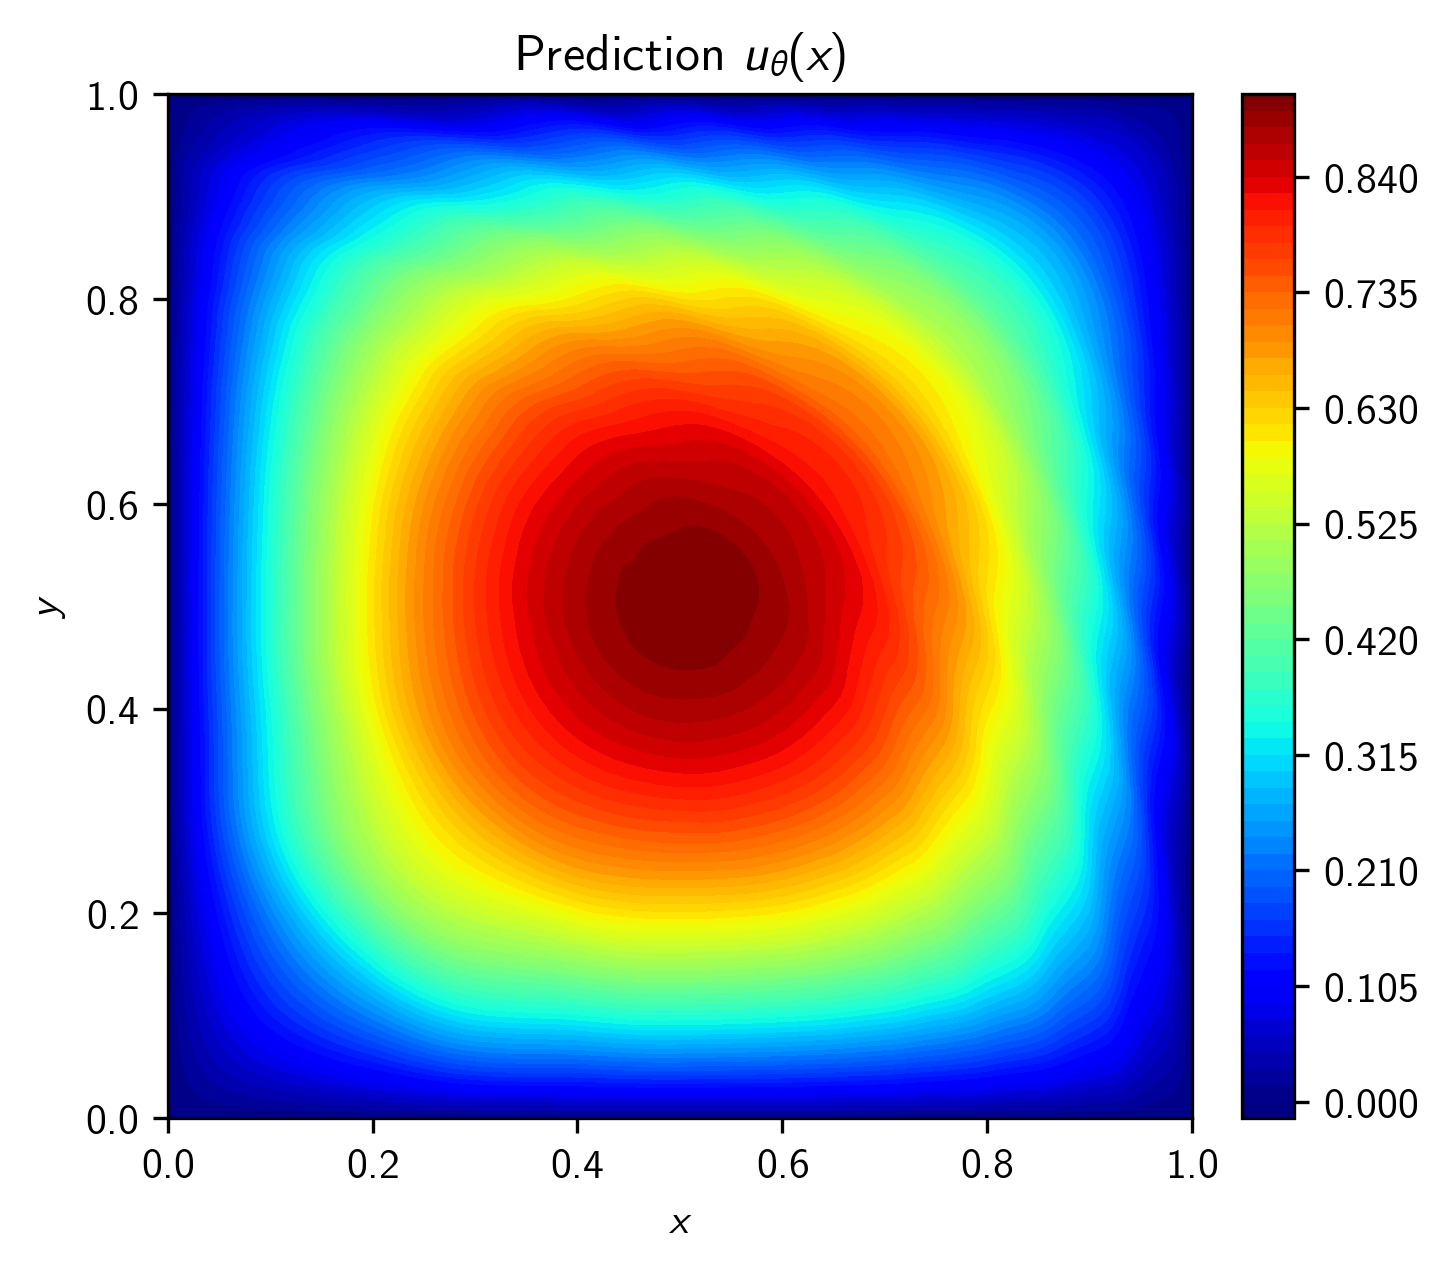
\includegraphics[width=\textwidth]{../Problem_C/predicted_u.png}
		\caption{Prediction $u_\theta(x,y)$}
	\end{subfigure}
	
	\vskip\baselineskip
	
	\begin{subfigure}[b]{0.495\textwidth}
		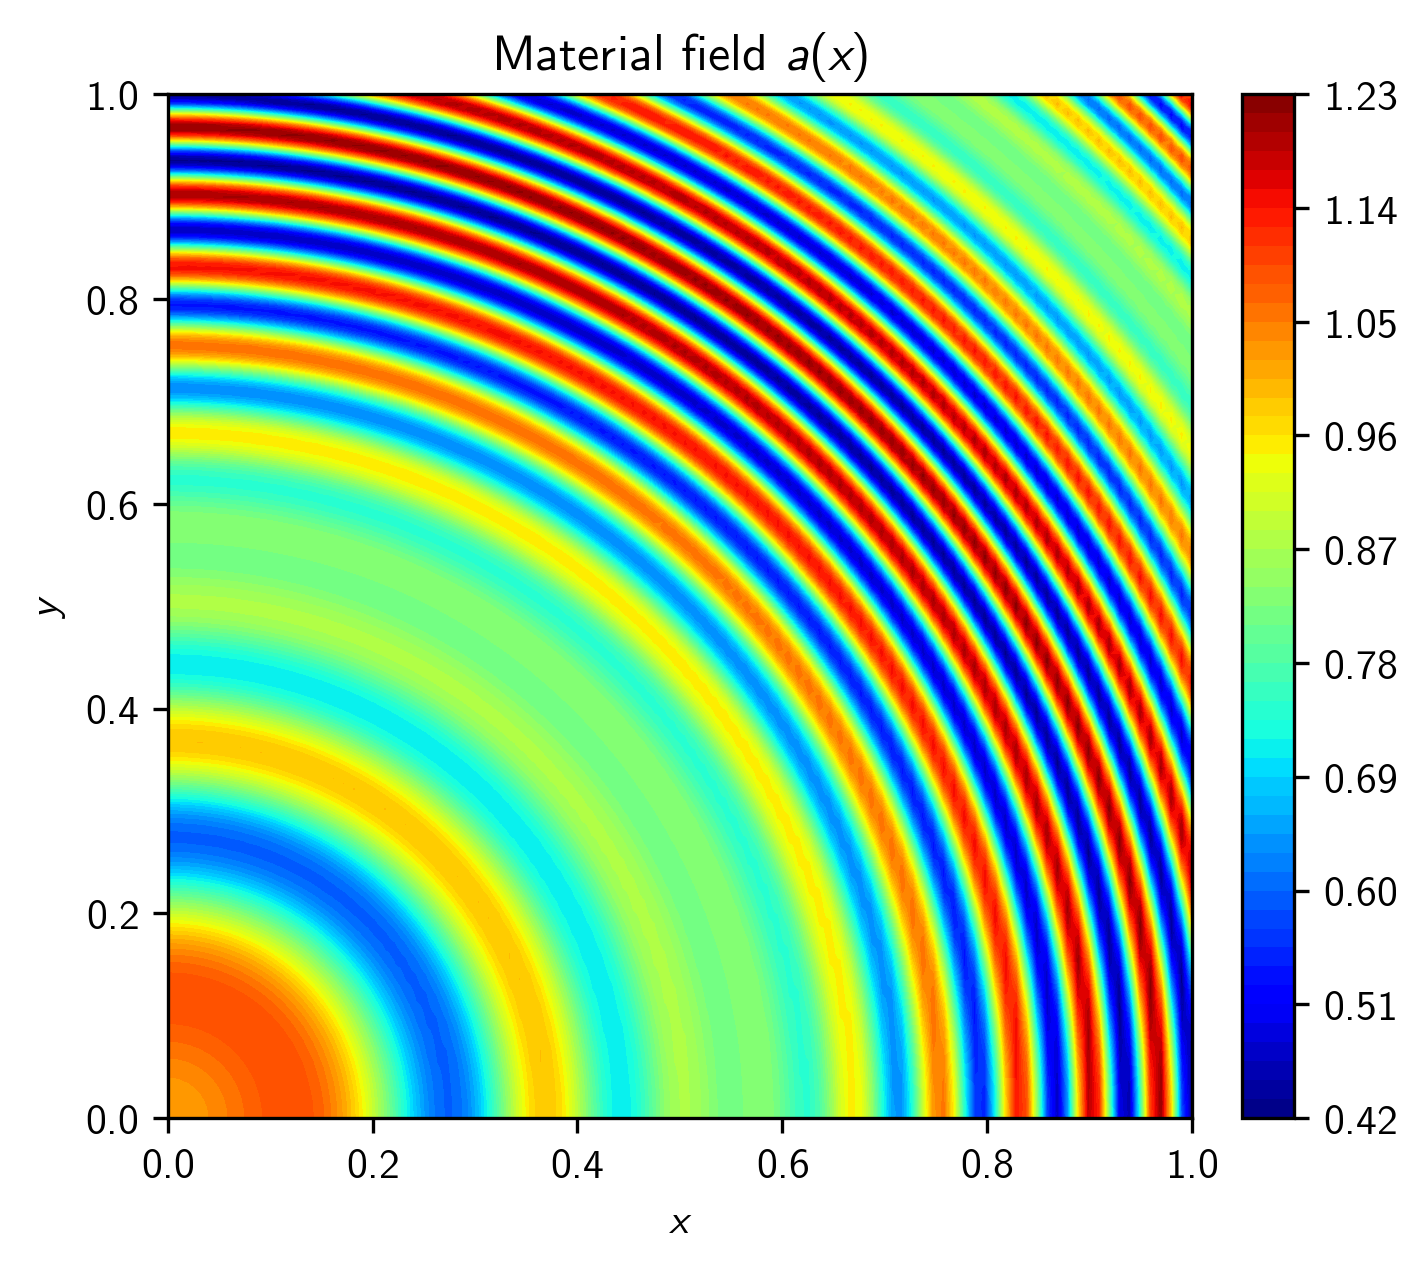
\includegraphics[width=\textwidth]{../Problem_C/input_a.png}
		\caption{Conductivity field $a(x,y)$}
	\end{subfigure}
	\hfill
	\begin{subfigure}[b]{0.495\textwidth}
		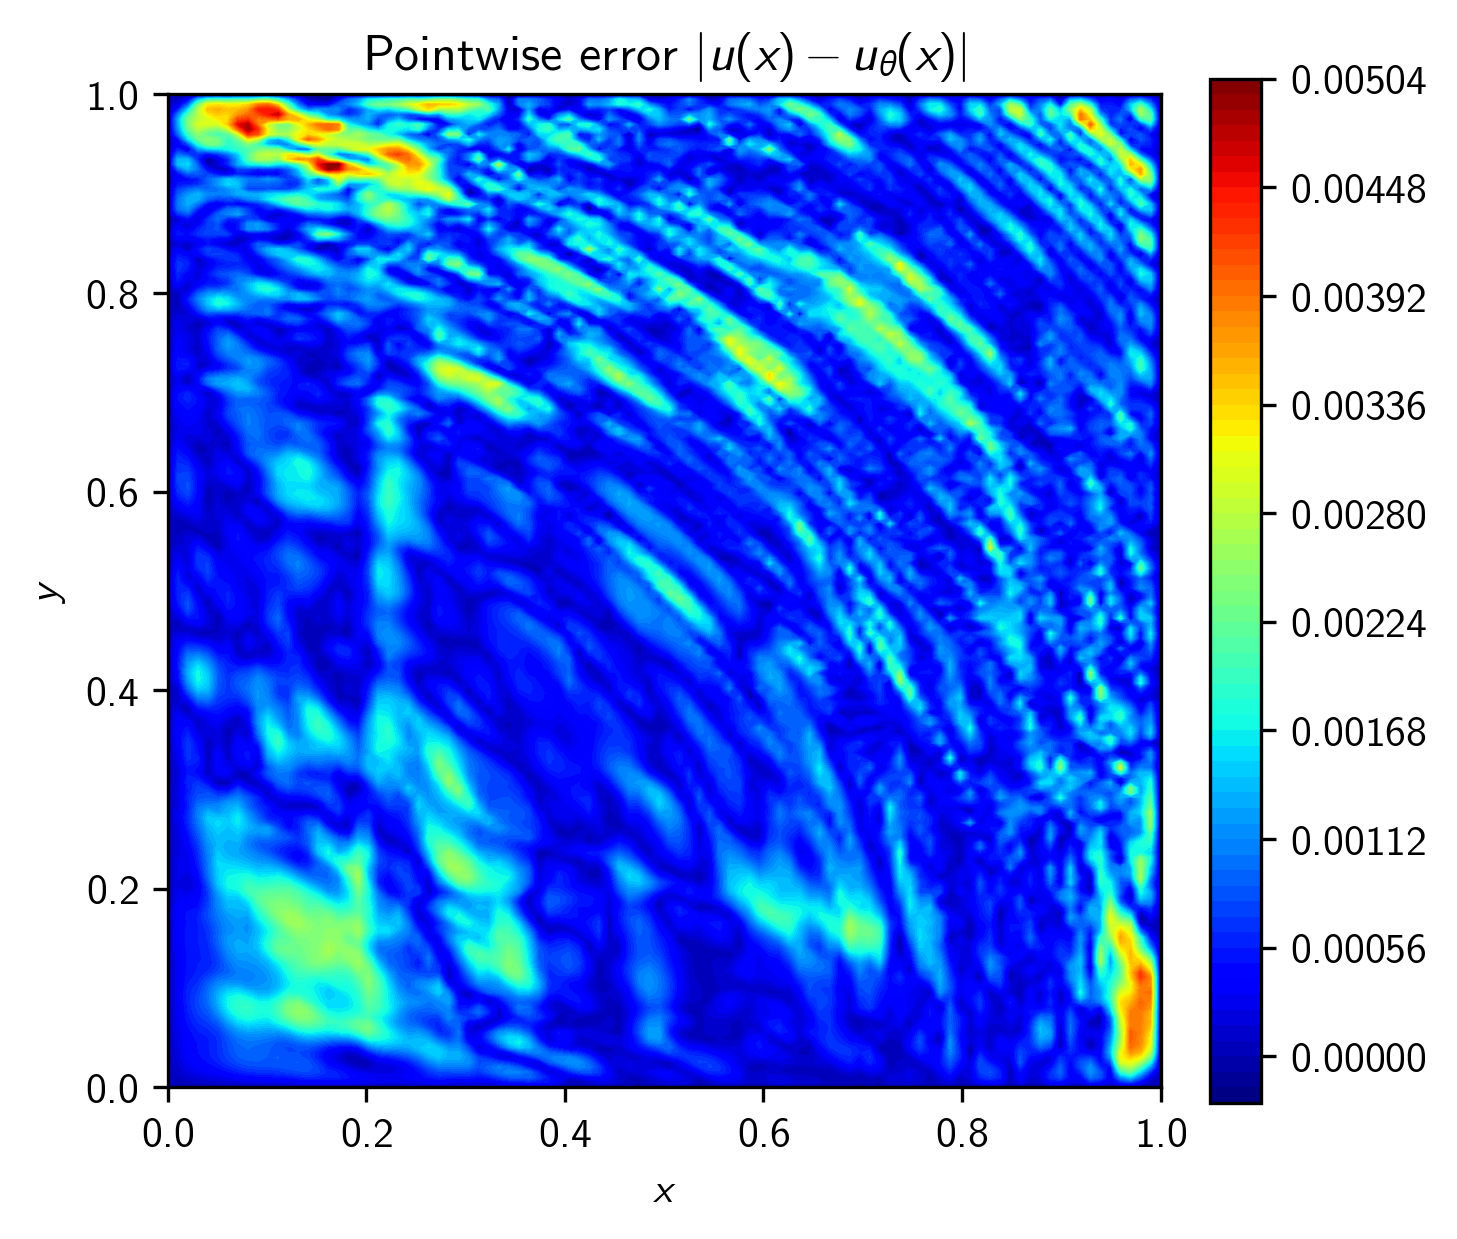
\includegraphics[width=\textwidth]{../Problem_C/pointwise_error_u.png}
		\caption{Pointwise error $|u(x,y) - u_\theta(x,y)|$}
	\end{subfigure}
	
	\caption{Experiment results for the first test instance of Problem C}
	\label{fig:problem_C_results}
\end{figure}




\begin{figure}[H]
	\centering
	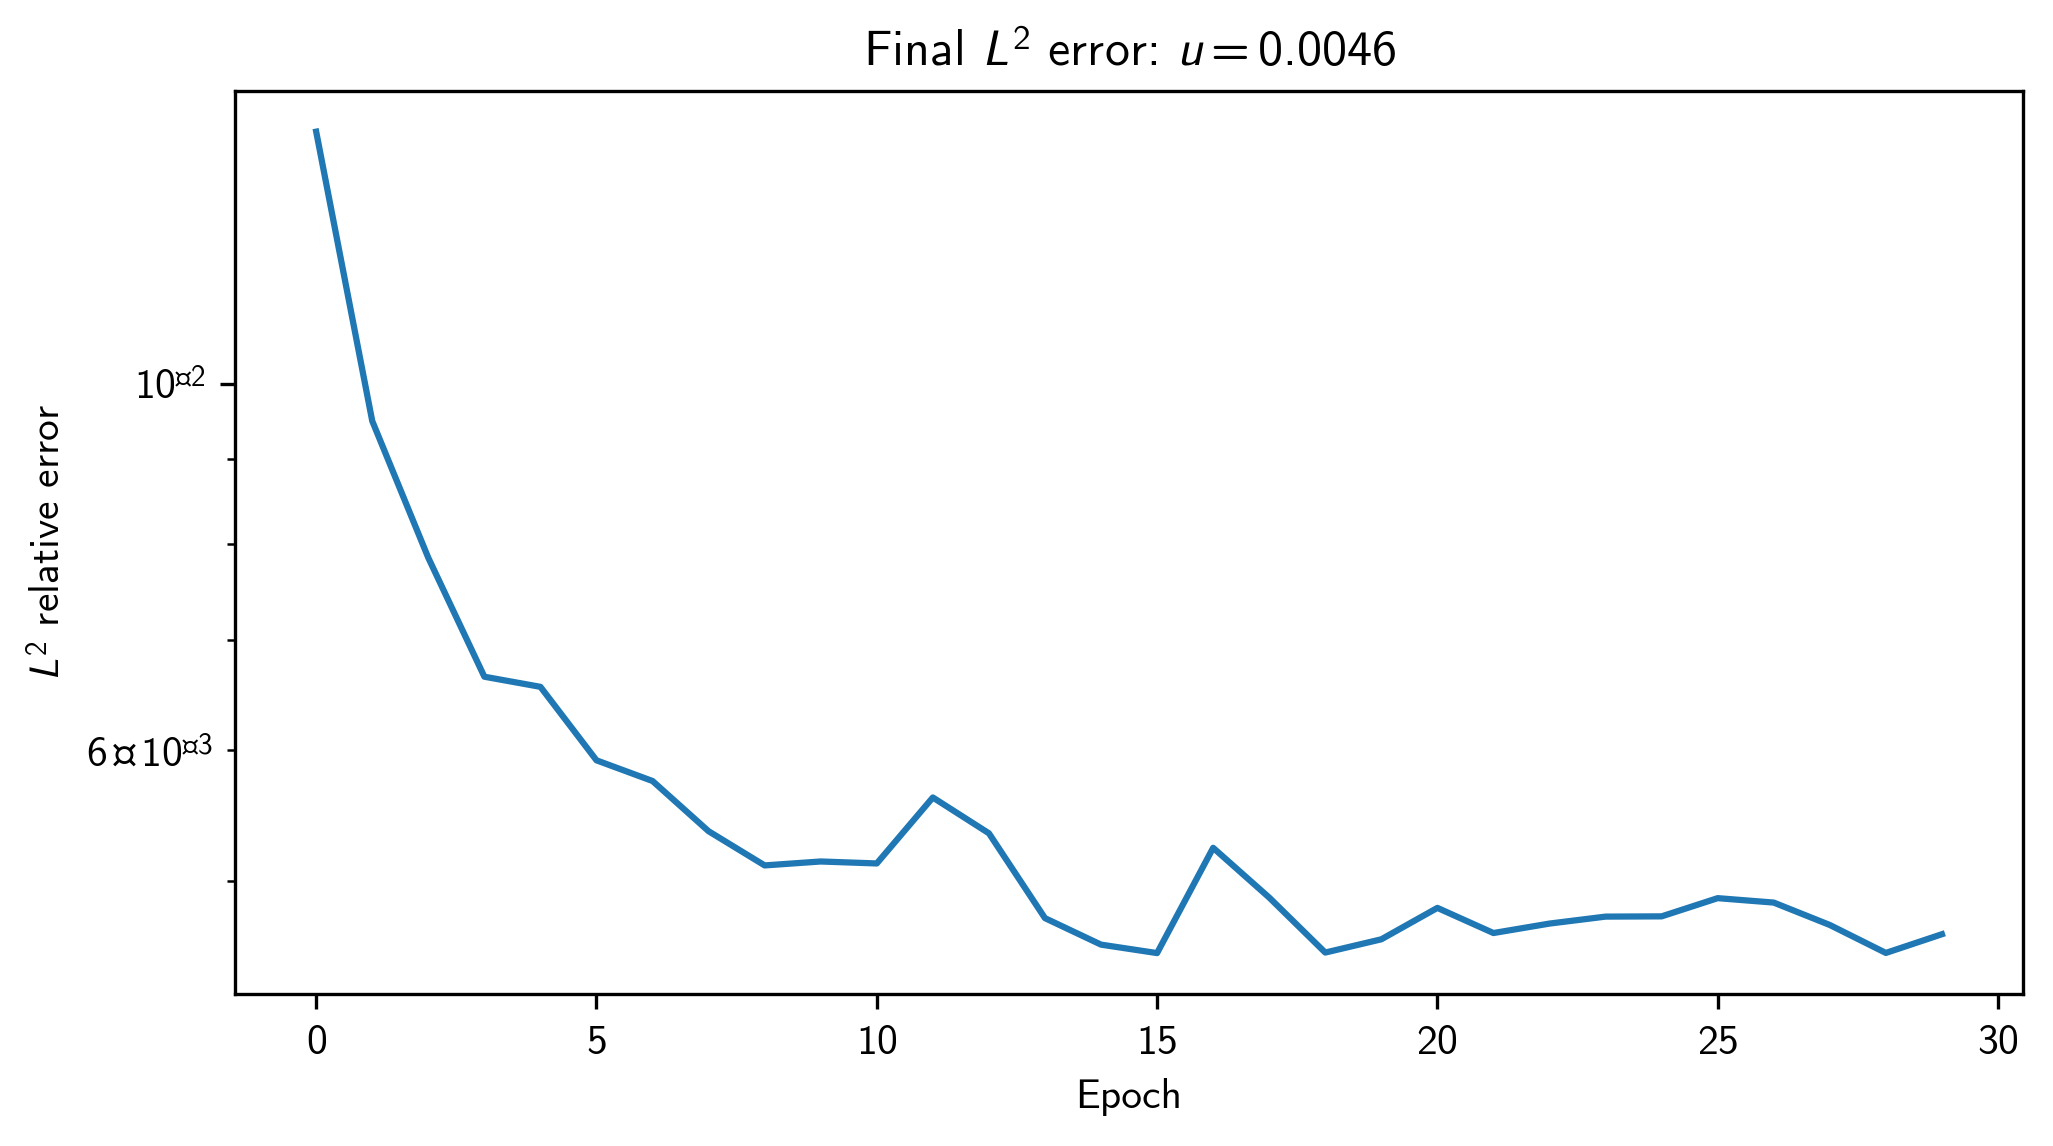
\includegraphics[width=0.8\textwidth]{../Problem_C/error_vs_epoch.png}
	\caption{Evolution of $L^2$ relative error for Problem C}
	\label{fig:problem_C_loss_history} 
\end{figure}



\subsection{Discussion}

As shown in Figure \ref{fig:problem_C_results}, the ground truth temperature field is approximated almost perfectly by the FNO. The absolute pointwise error achieved is mostly uniformly low, except for some regions where the conductivity field $a(x,y)$ has complex features. The conductivity field also has some patterns that are visually periodic/oscillatory, which the FNO excels at recognizing. This may be one of the reasons that the FNO works so well on this specific dataset.

Despite the training generally being slow (often reaching a few seconds per iteration), the $L^2$ relative error in Figure \ref{fig:problem_C_loss_history} appears to flatten out at just 20 iterations with the chosen hyperparameter set, meaning the convergence is rather fast. There do exist some oscillations in the curve, which implies that the model would benefit from more fine-tuning of the learning rate and its decay. This would likely lead to a lower final loss and thus a better performance.




%%%%%%%%%%%%%%%%%%%%%%%%%%%%%


\chapter{Problem D}
\label{ch:problem_D}
%
\section{Problem Description}
%

Problem D consists in predicting the velocity field $u(x,t)$ of a road segment with traffic flow given an initial velocity profile $u(x,0) = a(x)$. The governing PDE in this problem is Burgers' equation, namely

\begin{equation}
	\frac{\partial u}{\partial t} + u \frac{\partial u}{\partial x} = \nu \frac{\partial^2 u}{\partial x^2}, \quad x\in (-1,1), t\in (0,1]
\end{equation}

\noindent
where $\nu = 0.1/\pi$ is the kinematic viscosity coefficient.

In addition to the previously mentioned initial condition $a(x)$, the PDE is subject to homogeneous Dirichlet boundary conditions at both ends of the road for the entire duration of time:

\begin{equation}
	u(-1,t) = u(1,t) = 0, \quad t\in (0,1]
\end{equation}

The provided dataset is partially labeled, meaning that only some of the training examples $a(x)$ are paired with a corresponding ground truth solution field $u(x,t)$. Specifically, the dataset contains 200 labeled examples and 1800 unlabeled examples.

\section{Methodology}
%
\subsection{The method selection}
%Describe the method you use and the reason for choosing it.
%

Similarly to Problem C, this problem involves learning an operator $\mathcal{G}_\theta$ from an input field to a solution field. In this case the dataset is not fully labeled, so a physics-informed DNO approach is necessary in order to extract information from the entire dataset.

For this purpose, the Physics-Informed Fourier Neural Operator (PINO) is selected. The reason for choosing PINO over PI-DeepONet is that the latter requires implementing 2 networks (branh net and trunk net), while the former requires just 1. Hence it was deemed simpler to implement, in addition to having less hyperparameters to be tuned.




\newpage
\subsection{The loss function}
%Describe the loss function you use and the corresponding hyperparameters (i.e., loss weights, collocation points/integral points, and so on) used in training.
%   

The loss function for Problem D consists of a data loss computed using the labeled examples and a PDE loss computed using all training examples. The reason a boundary loss is not used is that the Dirichlet conditions are directly enforced via a "boundary-vanishing mask" $m(x)$ that is later multiplied with the raw output of the network $\hat u_\theta(x,t)$:

\begin{equation}
	m(x) = \cos\left( \frac{\pi x}{2} \right)
\end{equation}

Since the mask is 0 at $x = \pm 1$, the predicted solution $u(x,t)$ will also be 0 at those spatial locations. Next, this product is multiplied by time $t$ and added to the initial velocity profile $a(x)$ in order to also enforce that the initial condition is satisfied, as such:

\begin{equation} \label{eq:t_mask_u_hat}
	u_\theta(x,t) = a(x) + t \cdot m(x) \hat u_\theta(x,t)
\end{equation}

While this masking step is not strictly necessary for the network to function, it was found that the overall performance was improved, given that the network respects the boundary conditions from the very start of the training process.

The data loss is given by

\begin{equation}
	\mathcal{L}_\mathrm{data} = \frac{1}{N_\mathrm{lab}} \sum_{i=1}^{N_\mathrm{lab}} \left\Vert \mathcal{G}_\theta \left(a_i(x,y)\right) - u_i(x,y) \right\Vert_2
\end{equation}

\noindent
where $N_\mathrm{lab} = 200$ is the number of labeled training examples.

The PDE loss is computed as the mean of the sums of squared strong-form PDE residuals $\mathcal{R} \left[ u_\theta ; a \right]_{i,j}$ evaluated at all interior grid points for each sample in the batch. To approximate the derivatives in the residuals, central finite differencing is used, which is fast and consistent with PINO's grid-based representation:

\begin{equation}
	\mathcal{R} \left[ u_\theta ; a \right]_{i,j} =
	 \left. \frac{\partial u_\theta}{\partial t} \right|_{x_j, t_i} 
	 + u_\theta (x_j, t_i) \left. \frac{\partial u_\theta}{\partial x} \right|_{x_j, t_i}
	  - \nu \left. \frac{\partial^2 u_\theta}{\partial x^2} \right|_{x_j, t_i}
\end{equation}

\begin{align}
	\left. \frac{\partial u_\theta}{\partial t} \right|_{x_j, t_i} &\approx \frac{u_\theta(x_j, t_{i+1}) - u_\theta(x_j, t_{i-1})}{2\Delta t}\\
	\left. \frac{\partial u_\theta}{\partial x} \right|_{x_j, t_i} &\approx \frac{u_\theta(x_{j+1}, t_i) - u_\theta(x_{j-1}, t_i)}{2\Delta x}\\
	\left. \frac{\partial^2 u_\theta}{\partial x^2} \right|_{x_j, t_i} &\approx \frac{u_\theta(x_{j+1}, t_i) - 2 u_\theta(x_j, t_i) + u_\theta(x_{j-1}, t_i)}{2\Delta x^2}
\end{align}

The PDE loss is then given by

\begin{equation}
	\mathcal{L}_\mathrm{PDE}
	= \frac{1}{N_\mathrm{train} N_x N_t}
	\sum_{i=1}^{N_\mathrm{train}}\sum_{j,k}
	\left|\mathcal{R} \left[ \mathcal{G}_\theta (a_i); a_i \right]_{j,k}\right|^2
\end{equation}

\noindent
where $N_\mathrm{train} = N_\mathrm{lab} + N_\mathrm{unlab} = 200 + 1800 = 2000$ is the total number of training examples (labeled + unlabeled), $N_x = 256$ is the spatial resolution of the velocity field and $N_t = 200$ is the temporal resolution of the velocity field.

Finally, the total training loss $\mathcal{L}_\theta$ is the weighted sum of both losses, where the weights associated to each loss are hyperparameters.

\begin{equation}
	\mathcal{L}_\theta = w_\mathrm{data} \mathcal{L}_\mathrm{data} + w_\mathrm{PDE} \mathcal{L}_\mathrm{PDE}
\end{equation}


\subsection{The network structure}
%Describe the network structure that you use during training. 
%

In order to slightly facilitate the implementation of this PINO, the data for the initial velocity profiles $a(x)$ was extruded across the time dimension, resulting in 2-dimensional fields $a(x,t)$, as can be seen in Figure \ref{fig:problem_D_extrusion}. The reasoning for this choice was that this extrusion could provide information about the initial condition of the PDE to the network at every point in time, in addition to not requiring a change of shape during the lifting or projection steps. This way, the mapping is 2D to 2D.


\begin{figure}[H]
	
	\centering
	\begin{subfigure}[b]{0.41\textwidth}
		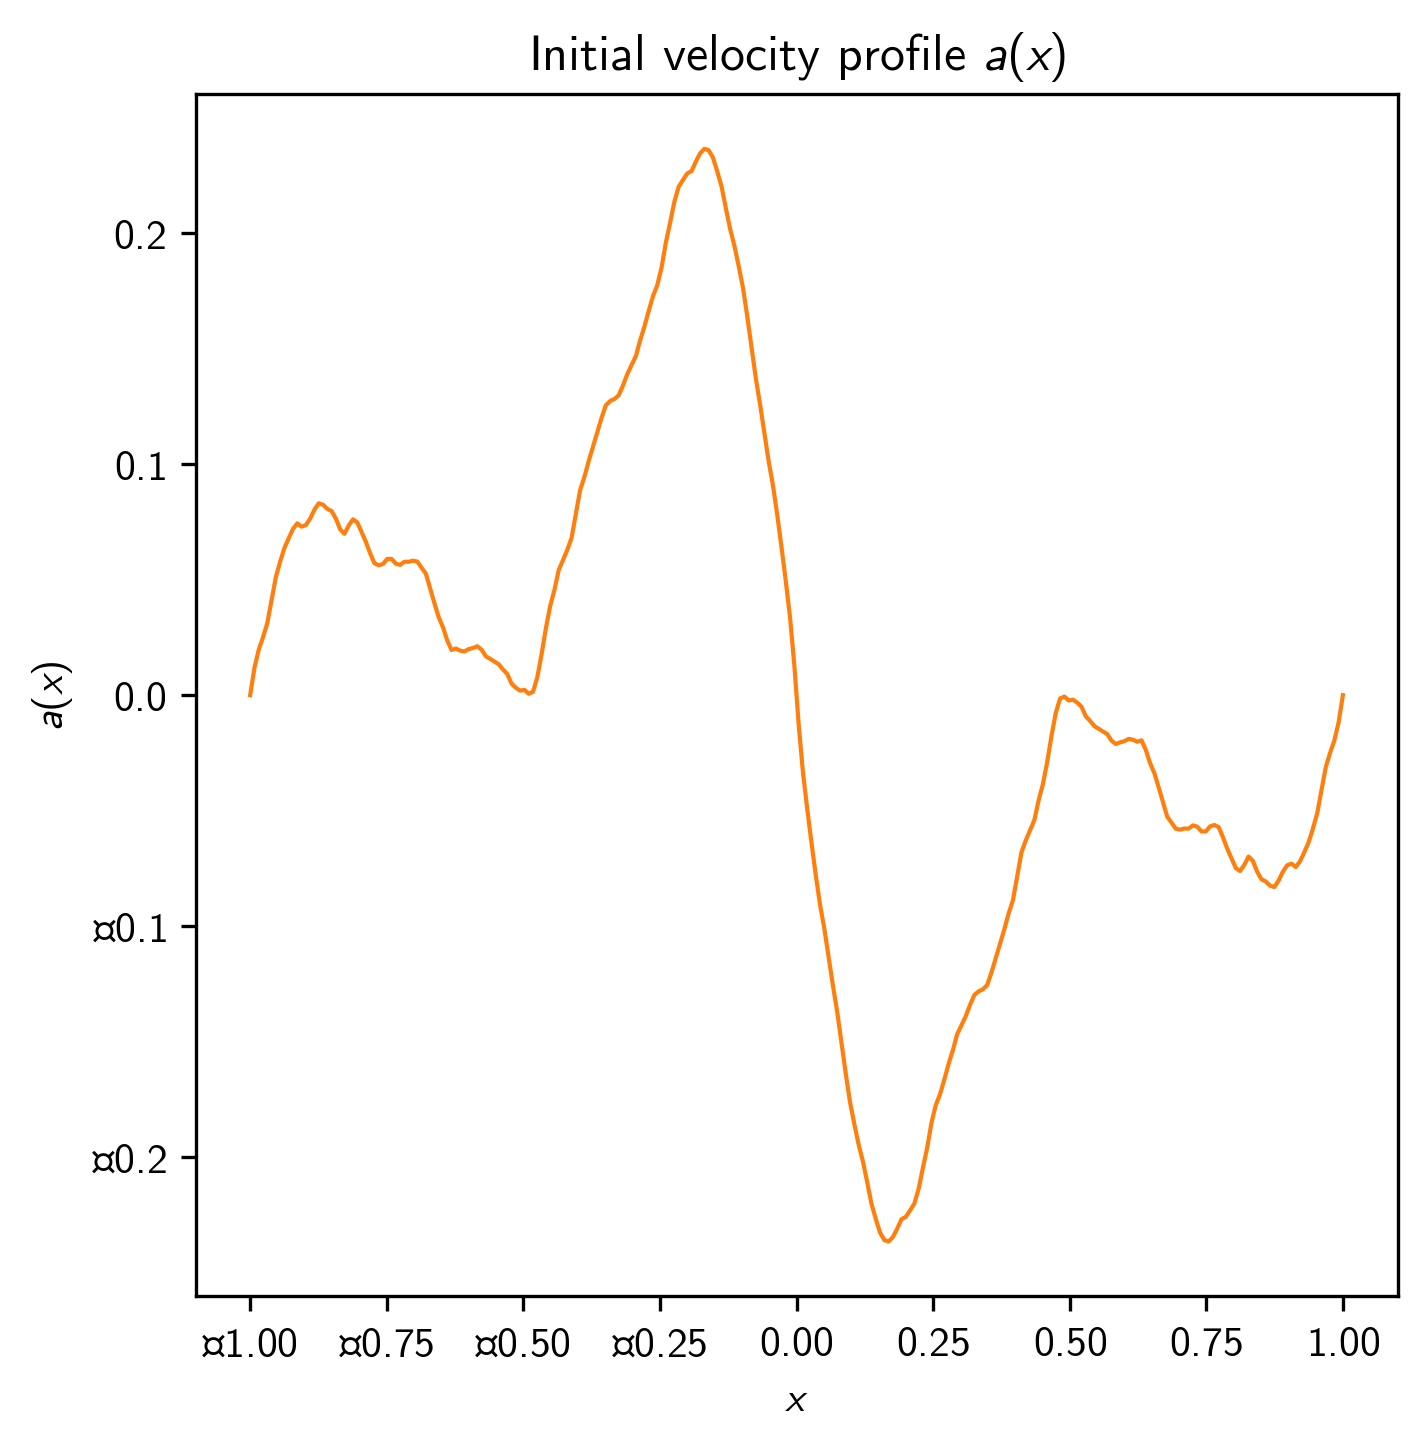
\includegraphics[width=\textwidth]{../Problem_D/input_a_1D.png}
		\caption{1D velocity profile $a(x)$}
	\end{subfigure}
	\hfill
	\begin{subfigure}[b]{0.5\textwidth}
		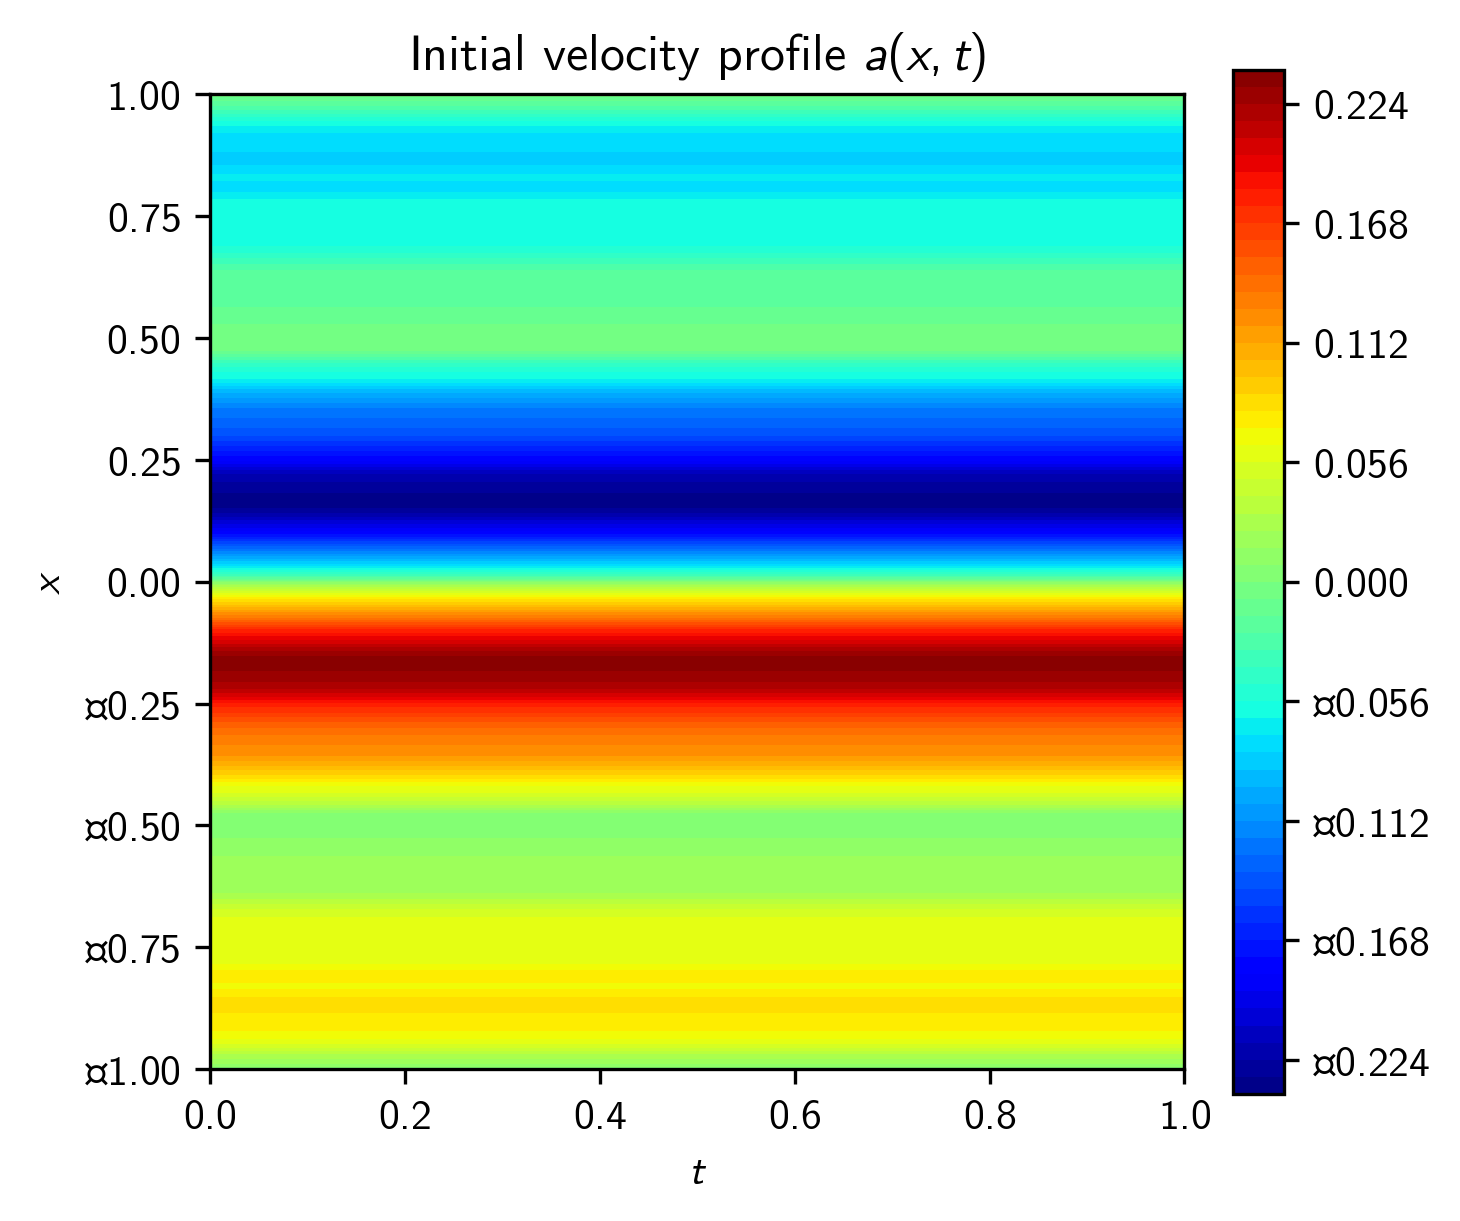
\includegraphics[width=\textwidth]{../Problem_D/input_a.png}
		\caption{Extruded 2D velocity profile $a(x,t)$}
	\end{subfigure}
	
	\caption{Extrusion of $a(x)$ to the time dimension}
	\label{fig:problem_D_extrusion}
\end{figure}


The network structure used for Problem D is conceptually identical to the one used in Problem C and described in Figure \ref{fig:problem_C_architecture}. Only some minor changes have been made to the size of the model, which are summarized in Table \ref{tab:problem_D_network}.


\begin{table}[H]
	\centering
	\caption{Network architecture of PINO for Problem D}
	\label{tab:problem_D_network}
	\begin{tabular}{llll}
		\hline
		\textbf{Layer} & \textbf{Size / Neurons} & \textbf{Activation Function} & \textbf{Notes} \\
		\hline
		Lifting Layer        & 20                                & Linear         & - \\
		Fourier Layer 1        & 20                                & $\sigma_D(x)$ = ReLU         & 8 modes used \\
		Fourier Layer 2     & 20                              & $\sigma_D(x)$ = ReLU       & 8 modes used \\
		Projection Layer 1     & 128                              & Linear       & - \\
		Projection Layer 2     & 128                              & ReLU       & - \\
		Projection Layer 2     & 1                              & Linear       & - \\
		\hline
	\end{tabular}
\end{table}

\subsection{The code link}
{\color{blue}Please provide the hyperlink (e.g., GitHub, Google Colab, or Kaggle Notebook) to your original code for solving this problem.} 
%
\section{Numerical Results}
%
\subsection{Experiment Setups}
%Describe the experiment setups for training the model.
%

The hyperparameters used in the experimental setup are listed in Table \ref{tab:training_setup_D}. 


\begin{table}[H]
	\centering
	\caption{Numerical setup for training the PINO in PyTorch}
	\label{tab:training_setup_D}
	\begin{tabular}{ll}
		\hline
		\textbf{Parameter} & \textbf{Value} \\
		\hline
		Optimizer           & Adam \\
		Learning Rate (initial)       & $5 \times 10^{-4}$ \\
		Weight Decay       & $1 \times 10^{-4}$ \\
		Batch Size          & 10 \\
		Number of Epochs    & 30 \\
		Learning Rate Scheduler & StepLR \\
		Decay Rate ($\alpha$/N epochs) &  0.9/10\\
		Hardware            & NVIDIA RTX 3050 Laptop (4GB) \\
		Precision           & Float32 \\
		Early Stopping      & No \\
		\hline
	\end{tabular}
\end{table}

\subsection{Numerical Results}
%Report the results (e.g., the time consumption and the $L^2$ relative error) you obtained in this section.

\begin{figure}[H]
	\centering
	\begin{subfigure}[b]{0.495\textwidth}
		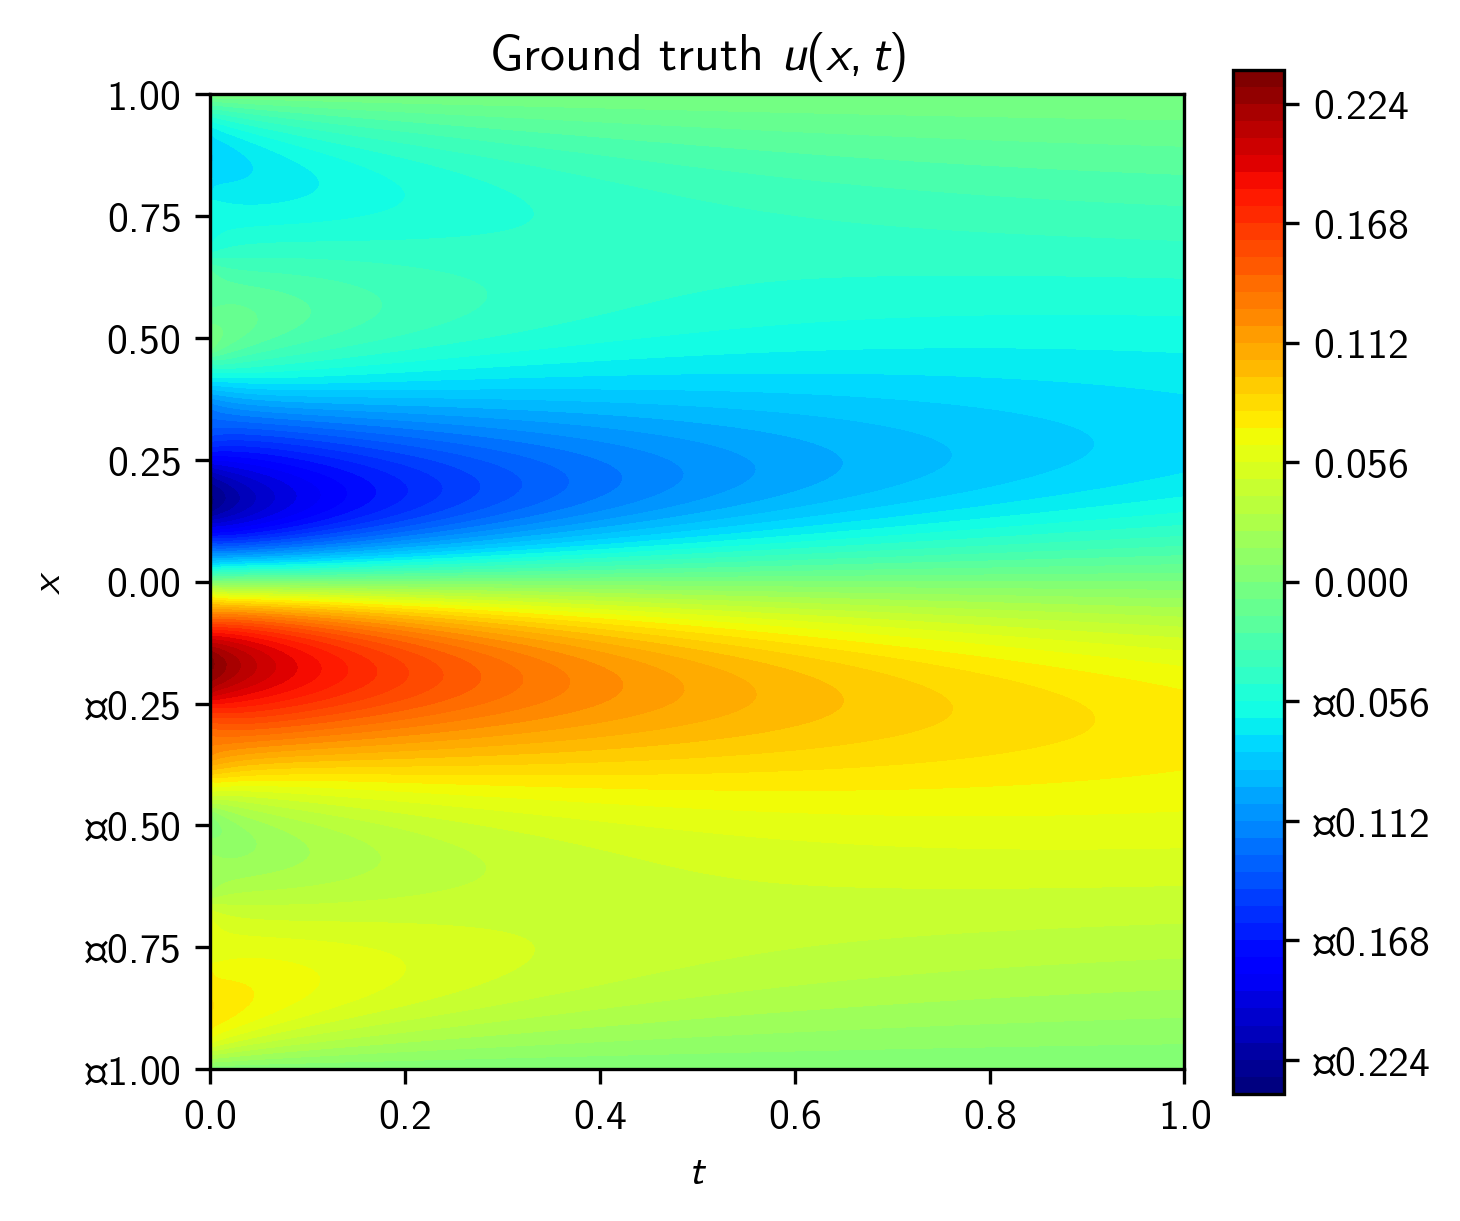
\includegraphics[width=\textwidth]{../Problem_D/GT_u.png}
		\caption{Ground truth $u(x,t)$}
	\end{subfigure}
	\hfill
	\begin{subfigure}[b]{0.495\textwidth}
		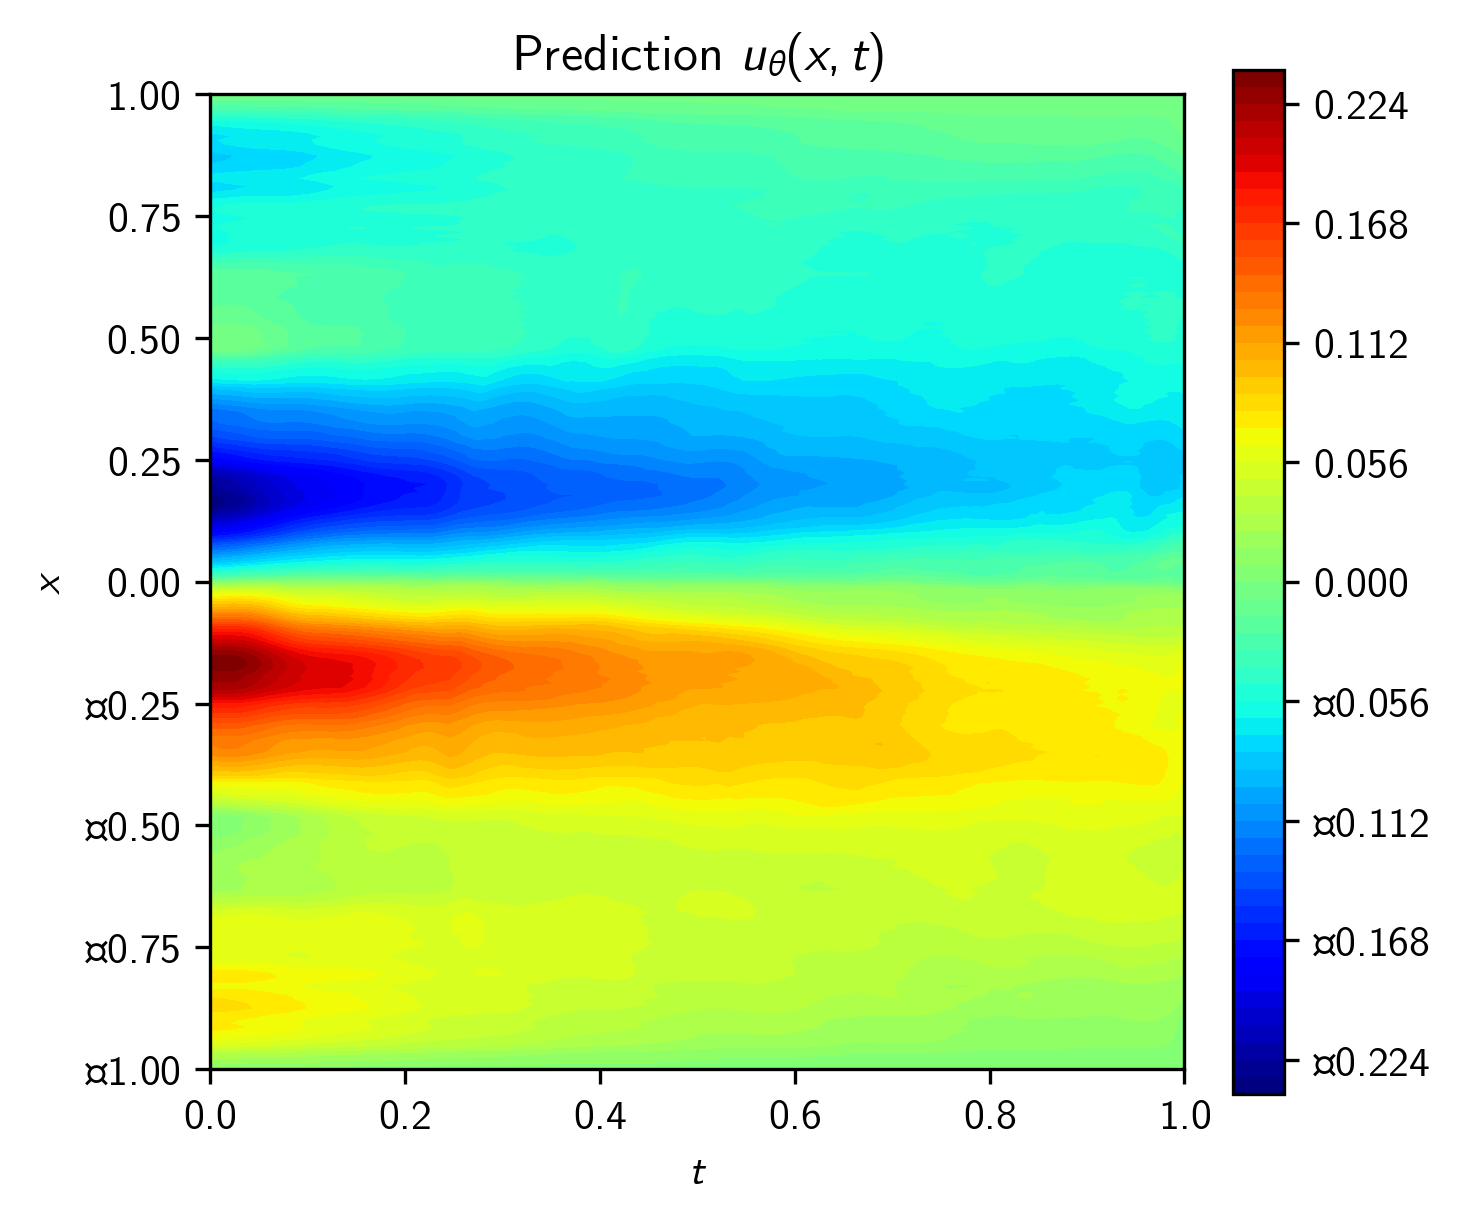
\includegraphics[width=\textwidth]{../Problem_D/predicted_u.png}
		\caption{Prediction $u_\theta(x,t)$}
	\end{subfigure}
	
	\vskip\baselineskip
	
	\begin{subfigure}[b]{0.41\textwidth}
		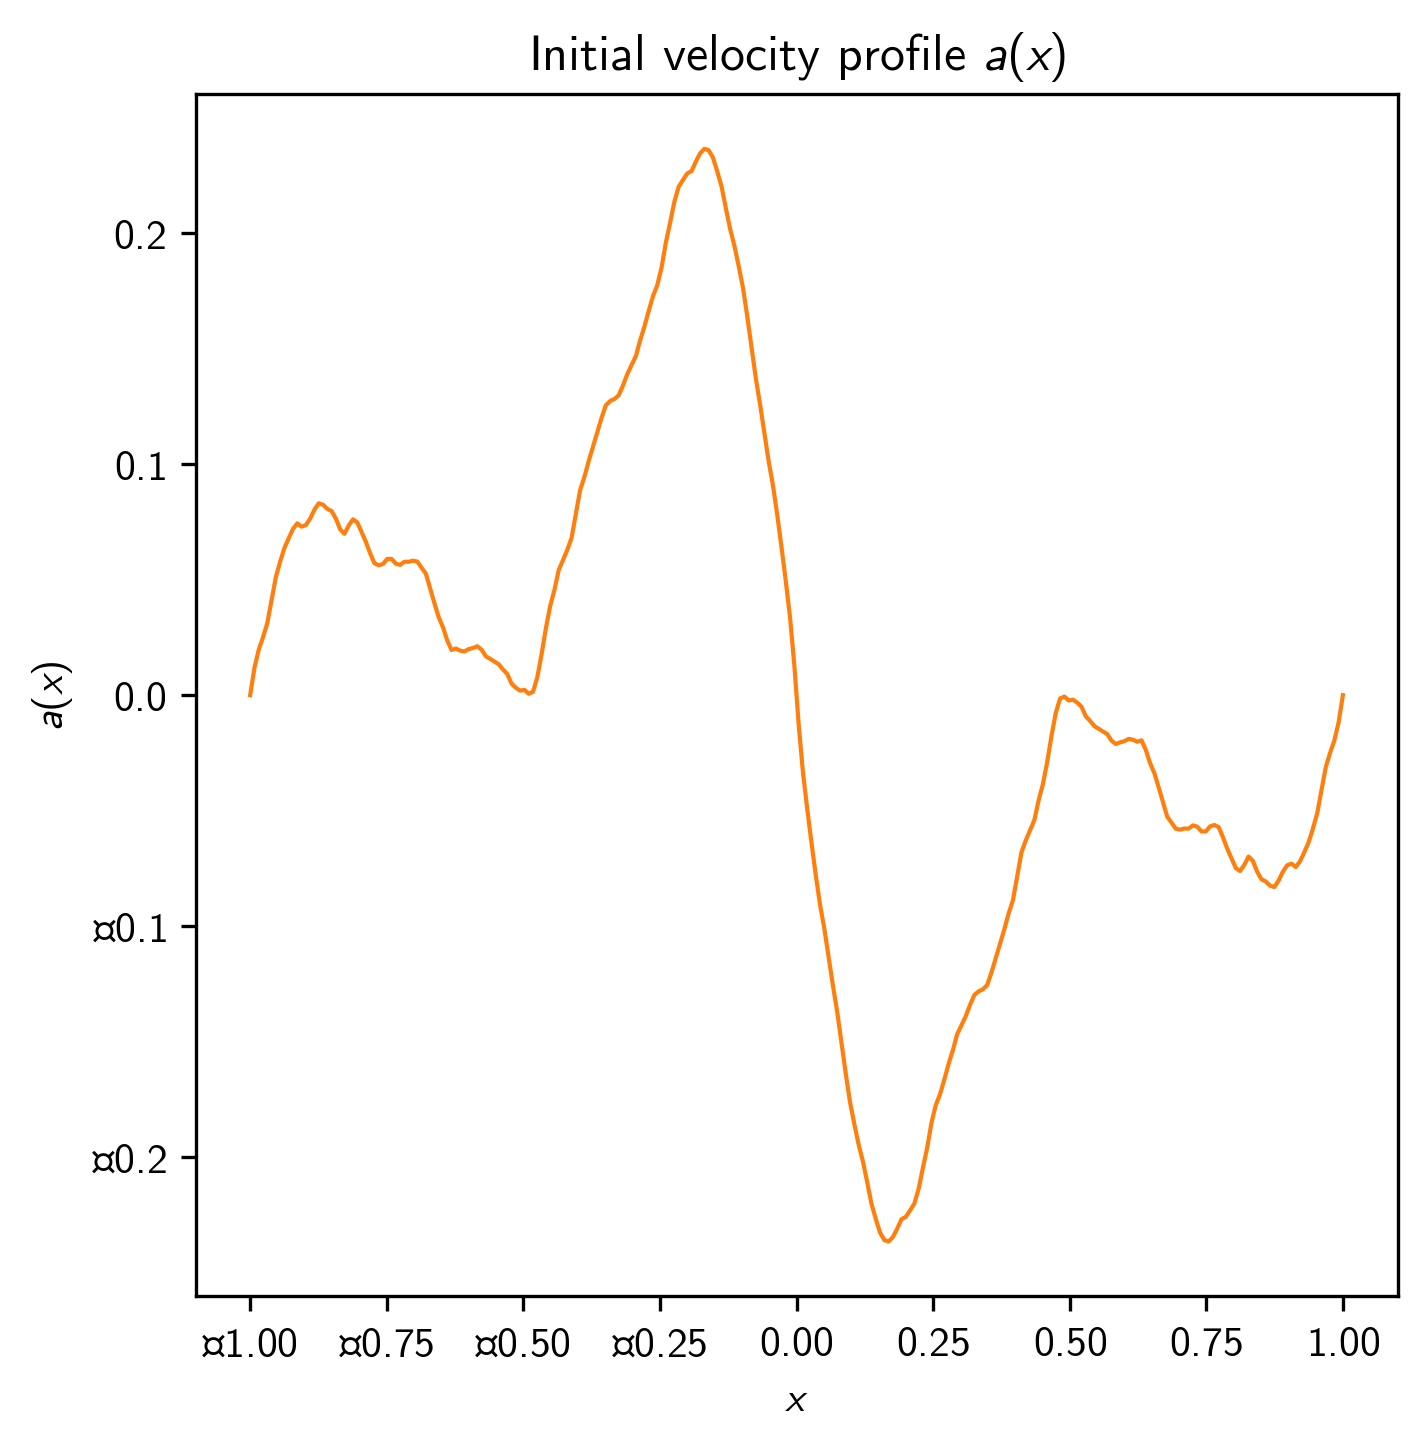
\includegraphics[width=\textwidth]{../Problem_D/input_a_1D.png}
		\caption{Initial velocity profile $a(x)$}
	\end{subfigure}
	\hfill
	\begin{subfigure}[b]{0.495\textwidth}
		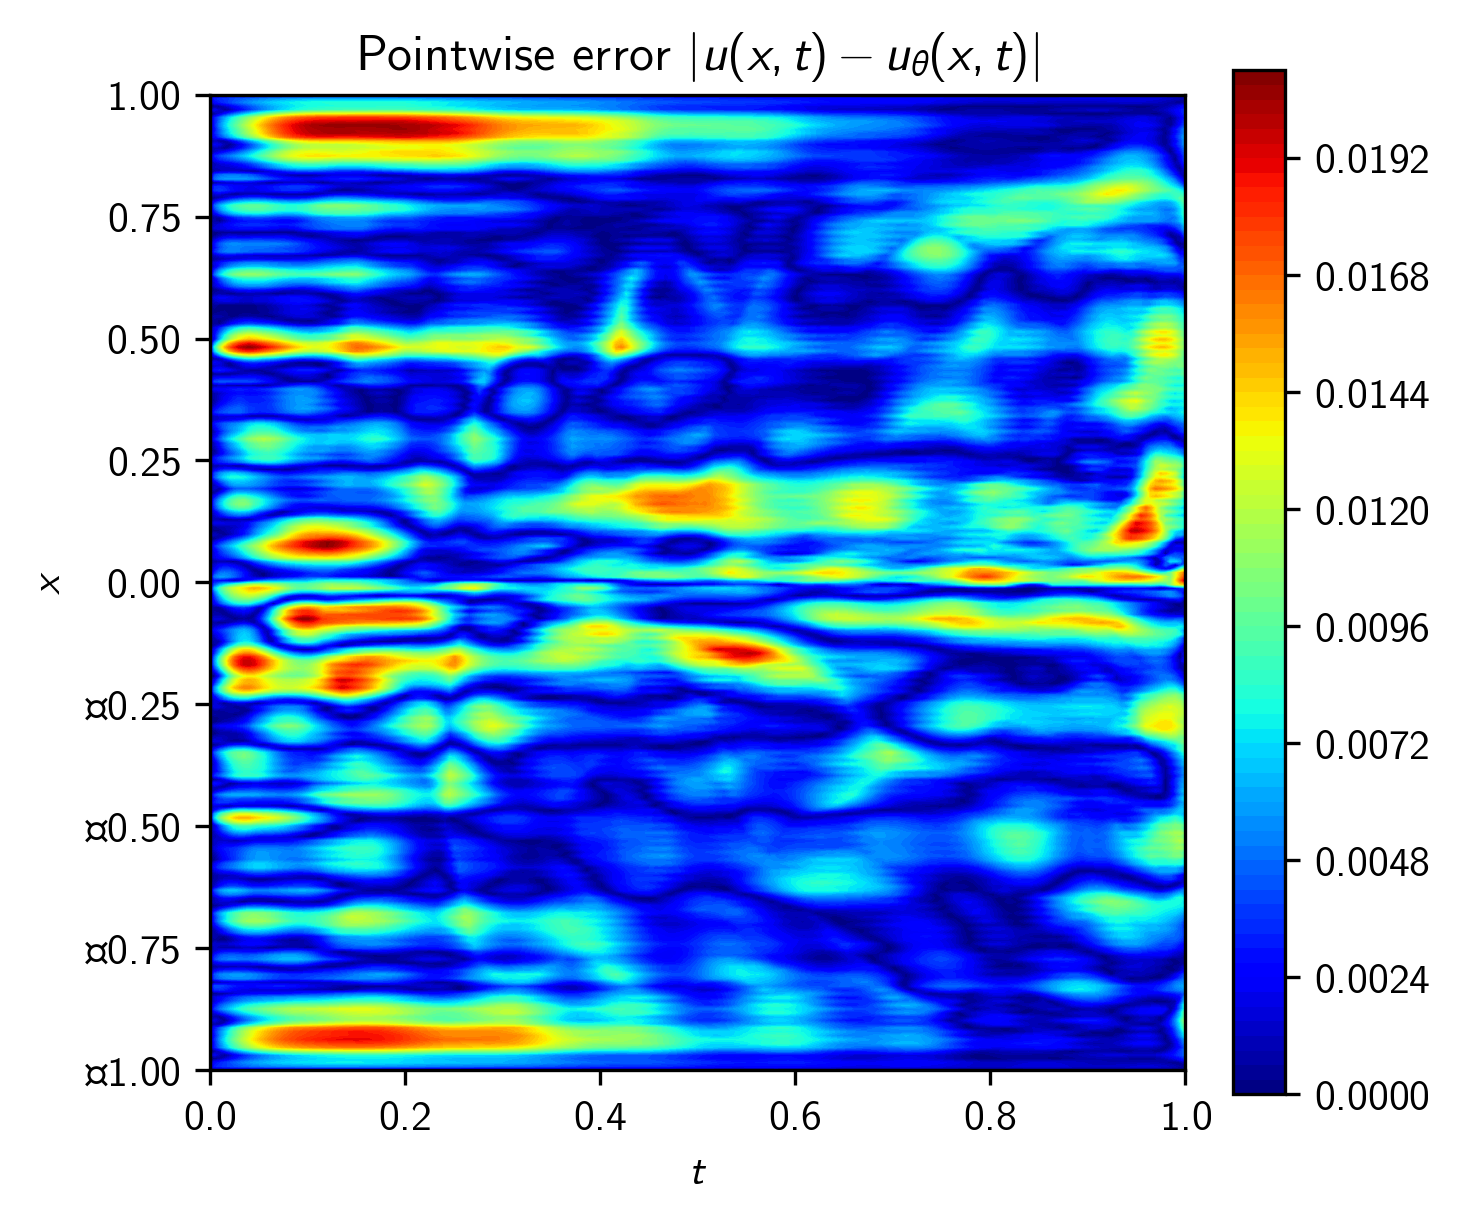
\includegraphics[width=\textwidth]{../Problem_D/pointwise_error_u.png}
		\caption{Pointwise error $|u(x,t) - u_\theta(x,t)|$}
	\end{subfigure}
	
	\caption{Experiment results for the first test instance of Problem D}
	\label{fig:problem_D_results}
\end{figure}




\begin{figure}[H]
	\centering
	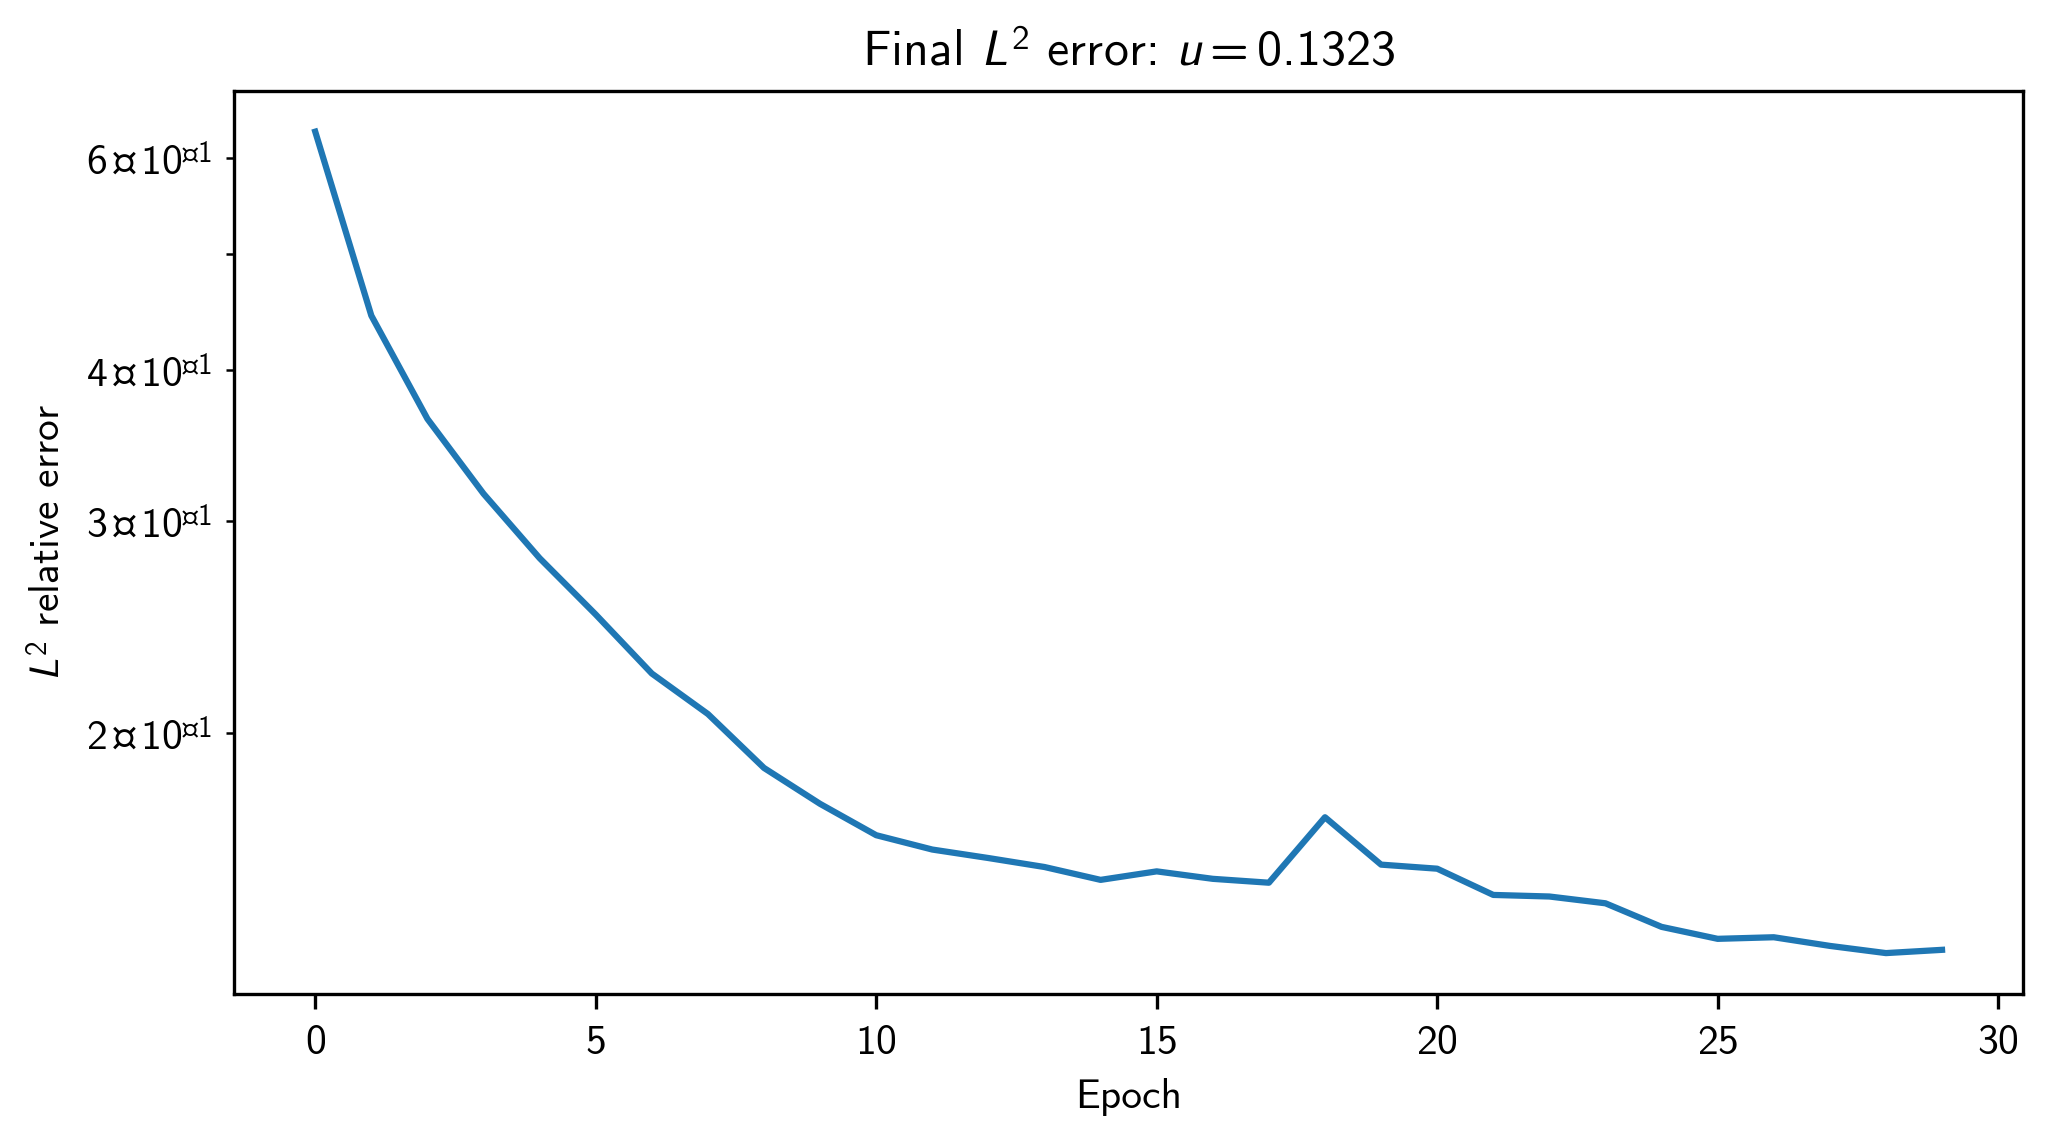
\includegraphics[width=0.8\textwidth]{../Problem_D/error_vs_epoch.png}
	\caption{Evolution of $L^2$ relative error for Problem D}
	\label{fig:problem_D_loss_history} 
\end{figure}



\subsection{Discussion}

As can be observed in Figure \ref{fig:problem_D_results}, the PINO does a good job at approximating the velocity field $u(x,t)$, primarily in terms of its overall shape and structure. The diffusive behavior is captured well, with the peaks and valleys in the spatial velocity profile smoothing out over time. As expected, the boundary conditions are perfectly respected, since this was forced to happen due to the application of the mask function in equation (\ref{eq:t_mask_u_hat}). However, the smoothness of the ground truth solution has not been completely captured, as the pointwise error field is somewhat noisy.

Similarly to the regular FNO used for Problem C, the training process for the PINO was very slow, but converged in as little as 30 epochs, as we can observe in Figure \ref{fig:problem_D_loss_history}. This time the convergence is smoother, hinting at well-tuned learning rate parameters. With the current number of epochs the $L^2$ relative error is just starting to flatten out, meaning the model may get some increase in performance by training it for longer, though this increase may not be significant.



